\documentclass[11pt]{article}
\usepackage[margin=1in]{geometry}
\usepackage{amsmath,amssymb,amsthm,mathtools,bm}
\usepackage{graphicx,booktabs,longtable,array,microtype,enumitem}
\usepackage[authoryear,round]{natbib}
\usepackage[colorlinks=true,allcolors=blue]{hyperref}
\newtheorem{theorem}{Theorem}
\newtheorem{proposition}[theorem]{Proposition}
\newtheorem{lemma}[theorem]{Lemma}
\newtheorem{corollary}[theorem]{Corollary}
\theoremstyle{definition}
\newtheorem{definition}[theorem]{Definition}
\theoremstyle{remark}
\newtheorem{remark}[theorem]{Remark}
\newcommand{\R}{\mathbb R}
\newcommand{\E}{\mathbb E}
\newcommand{\PP}{\mathbb P}
\newcommand{\ip}[2]{\langle #1,#2\rangle}
\newcommand{\norm}[1]{\lVert #1\rVert}
\newcommand{\Th}{\Theta}
\newcommand{\one}{\mathbf 1}
\newcommand{\tn}{t_n}
\newcommand{\pr}{\textsc{Proved}}
\DeclareMathOperator{\rank}{rank}
\DeclareMathOperator{\dist}{dist}
\DeclareMathOperator{\vecop}{vec}
\DeclareMathOperator{\TV}{TV}
\DeclareMathOperator{\KL}{KL}
\setlength{\emergencystretch}{3em}
\setlist{nosep}
\graphicspath{{figures/}}
\bibliographystyle{plainnat}

\title{Contact Orders and the Fragility of Honest Tensor Inference}
\author{Research draft for author review}
\date{8 September 2026: audited revision}
\begin{document}
\maketitle
\begin{abstract}
A linear functional of a tensor coefficient can have several vanishing derivatives on a rank-constrained model. We study globally honest inference in Gaussian tensor regression with fixed ambient dimension. At original-mode rank-one signals, cuts with tensor-train rank cap one partition the modes into blocks. We prove a local modulus formula that retains every orthogonal loading degree, uniformly over loadings and signal directions. The resulting optimal pointwise expected interval length describes transitions between regular and degenerate functionals, including loadings that vary with sample size. For a fixed loading of first nonzero degree $q$, the scale reduces to $(\sigma/\sqrt n)^q/\lambda^{q-1}$, with radial degree treated as first order. A known coefficient neighborhood adds $\norm A\min\{\eta,\sigma/\sqrt n\}$. A computable HOSVD confidence-ball certificate attains these orders, with an exact unknown-variance version and simultaneous coverage over contrasts. An energy refinement shortens the original certificate on every dataset. We separate geometric inference from localization, extending the analysis to quantitative non-Gaussian design conditions and retaining the full contact rate with a median-based localizer under independent observations and a known conditional variance bound. Simulations approach the predicted exponents and illustrate local Wald failure; a separate paired study confirms the certificate improvement while documenting remaining conservatism. The contribution is the constrained tensor modulus and its inferential consequences, rather than generic higher-order inference or a new modulus lower-bound principle.
\end{abstract}
\noindent\textbf{Keywords:} confidence intervals; tensor train; local modulus; singular inference; model approximation; higher-order contact.

\section{Introduction}
Structural restrictions can reduce uncertainty about a regression functional by more than a variance constant. Consider a four-way coefficient $B\in\R^{2\times2\times2\times2}$ whose TT rank caps are $(1,2,1)$. The outer rank-one cuts force a product of blocks of dimensions $(2,4,2)$. At $B_0=\lambda E_{0000}$, the coordinate functional $B\mapsto B_{1111}$ changes only when all three blocks change. A perturbation of Frobenius size $t$ can change this functional by order $t^3/\lambda^2$. This raises a statistical question: can an interval exploit that cubic behavior while retaining coverage over the whole rank-constrained class, including neighboring rank strata?

Existing theory makes a simple higher-order calculation insufficient as a contribution. Functional inference under degeneracy, including corrected bootstrap and minimum-distance methods, is well developed \citep{chenfang2019,bei2026}. Tensor inference with nondegenerate tangent alignment also has strong guarantees \citep{xu2025,maxia2024}. What requires a separate calculation here is the local modulus across a specified collection of TT constraints and the corresponding expected length under global honesty. In addition, structural rank restrictions may be approximate, and a small coefficient departure can be larger than a higher-order inferential scale.

We therefore study a deliberately explicit experiment: independent isotropic Gaussian designs, independent Gaussian regression errors, and a fixed-dimensional coefficient in a bounded TT rank class or a known neighborhood of that class. The main length estimand is a prespecified linear functional of the coefficient, not an individual TT core, a training-trajectory statistic, or an unobserved neural-network parameterization. Our main objective is to classify the best expected interval length at rank-one coefficients subject to coverage for every coefficient in the declared class. We allow unknown error variance but do not claim inference when ambient least squares is unavailable.

Three obstacles distinguish the calculation from a direct delta-method exercise. First, a path in an enclosing product model may violate an internal TT rank cap, so a lower modulus bound requires an actually feasible tensor path. Second, a confidence interval calibrated at the exact boundary can fail under statistically indistinguishable local changes, as Figure~\ref{fig:activation} illustrates. Third, the fitted loading projections have lower-order components even when the true ones vanish; these terms and the event of poor pilot localization must be controlled to bound expected length.

The construction uses the cuts whose rank cap equals one to partition the tensor chain. Orthogonal loading components are graded by the number of blocks perpendicular to the signal. For a fixed loading, the smallest nonzero degree determines the modulus exponent. Retaining all degrees gives a uniform formula when low-degree components approach zero. Within-block sums of two elementary products provide feasible witness paths despite the remaining TT constraints. Averaging signed paths isolates each degree without cancellation from lower ones. Confidence-ball inversion then supplies global coverage, while a graded product bound makes the calculation explicit. In the four-way example this recovers cubic inference. A six-way example with a proper singular internal rank constraint has the same cubic order, demonstrating both the scope of the classification and the limited role of that singularity.

The paper makes three claims, each proved in the appendix:
\begin{enumerate}
 \item Section~\ref{sec:theory} classifies local contact and optimal honest expected length at rank-one signals for arbitrary positive TT cap profiles, uniformly over deterministic loadings. It also shows that slack at every cut restores first-order contact for every nonzero loading.
 \item Theorem~\ref{thm:length} determines the additional length required by a known structural approximation allowance and identifies departures that cannot be detected but invalidate exact-model lengths.
 \item Section~\ref{sec:method} gives a computable, globally honest interval that attains these orders without selecting the contact order. The improved energy certificate is no longer than the original on any dataset. Section~\ref{sec:extensions} separates localization assumptions from geometry; experiments test the rate transitions, coverage distinction, and approximation sensitivity.
\end{enumerate}

\begin{figure}[t]
\centering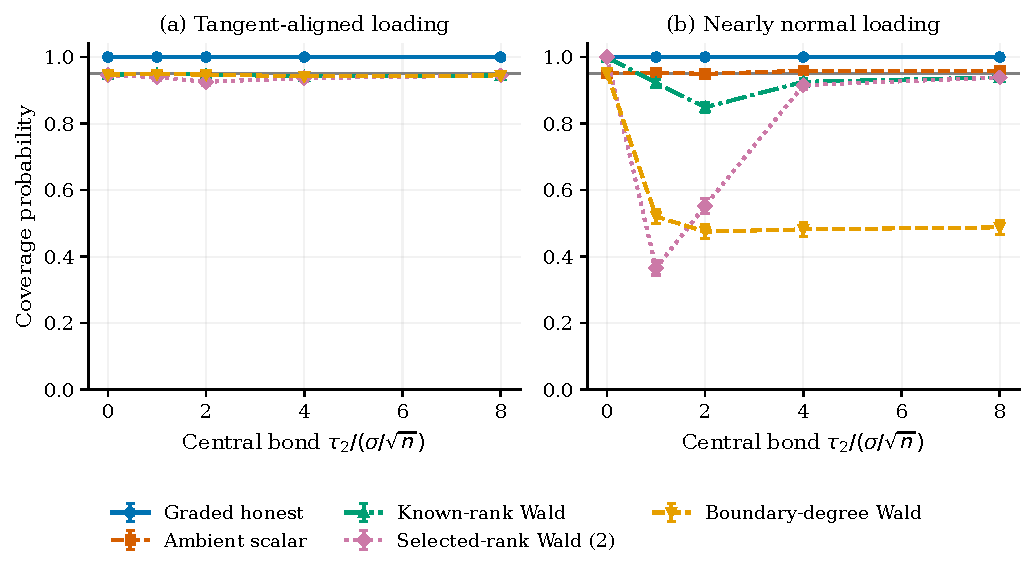
\includegraphics[width=\textwidth]{activation.pdf}
\caption{Exact-boundary calibration can fail under a local change in the central TT bond. Four binary modes have caps $(1,2,1)$, $n=2048$, $\lambda=3$, and $\sigma=0.2$; the path and two fixed loadings are specified in Section~\ref{sec:experiments}. Points use 2,000 replications with Wilson 95\% Monte Carlo intervals; the horizontal line is nominal coverage 0.95. ``Selected-rank Wald (2)'' uses the prespecified threshold multiplier two.}\label{fig:activation}
\end{figure}

\section{Related work and the scope of the contribution}
\paragraph{Degenerate functionals and singular tests.}
\citet{chenfang2019} develops second-order functional inference and explains ordinary-bootstrap failure; higher-order extensions are explicitly discussed. \citet{dufour2025} studies locally singular polynomial Wald restrictions. \citet{pillaimeng2016} gives the exact Gaussian monomial Wald law, including the cubic $\chi_1^2/9$ case. \citet{bei2026} constructs uniformly valid minimum-distance inference under degeneracy and discusses extensions beyond a nonsingular Hessian. These results preclude novelty claims based solely on a cubic delta method or a nonstandard Wald limit. Our explicit local Wald calculation is a supporting specialization of that literature.

\paragraph{Moduli, curved models, and model neighborhoods.}
The connection between honest interval length and between-class moduli is central to \citet{cailow2004}. Its lower-bound logic applies to singleton evaluation classes and does not require a new tensor information inequality. \citet{andrews2016} already obtains conservative inference from curved-model geometry. Model-misspecification sensitivity is studied by \citet{bonhomme2022}, and bias-aware intervals and efficiency comparisons by \citet{armstrong2021,armstrong2023}. Our neighborhood calculation uses the elementary modulus sandwich; the specific input is the classified TT contact order. We do not claim a new general theory of robust confidence intervals.

\paragraph{Rank uncertainty and tensor inference.}
\citet{carpentier2018} shows that rank-adaptive matrix confidence sets can exist, with feasibility depending on the observation and noise experiment. \citet{armstrong2026} allows weak factors in panel inference. Thus rank uncertainty is not a universal impossibility mechanism. In regular tensor settings, \citet{xu2025} and \citet{maxia2024} obtain functional Gaussian limits under signal, initialization, and nondegenerate alignment conditions. Their dimensions can increase, and their regular-regime results are stronger than the fixed-dimensional analysis here in that respect. We address a different boundary regime rather than improving their sample complexity. \citet{xia2022} also establishes important tensor inference results without a universal need for debiasing.

\paragraph{Tensor geometry, estimation, and computation.}
\citet{kutschan2018} characterizes TT tangent cones, and \citet{yang2025} gives first- and second-order variational formulas for determinantal tensor formats. Higher block-degree spans for product varieties appear in the osculating geometry of \citet{araujo2019}. We use that grading and verify feasible lower-bound paths inside the additional TT constraints. TT regression estimation and algorithmic guarantees are already supplied by \citet{qin2025}; oracle tensor regression under separation is studied by \citet{wang2025}. The spectral-norm hardness observation in Proposition~\ref{prop:hardness} inherits the result of \citet{hillarlim2013}; it is not an independent complexity theorem.

\paragraph{Finite-variance localization.}
Robust mean estimation with finite second moments is developed by \citet{devroye2016,lugosi2019}. Our coordinate-median OLS argument uses the classical independent-group amplification principle, then transfers the resulting radius moments through the TT modulus. It does not improve the dimension or confidence-level dependence of those mean-estimation results. The need to restrict a fully nonparametric unknown-noise class is consistent with the impossibility literature originating with \citet{bahadur1956}; the explicit regression construction in Appendix~\ref{app:counterexamples} is proved directly.

\paragraph{Modern tensor models and other inferential targets.}
Tensor regression networks \citep{kossaifi2020}, global rank-adaptive TT adapters \citep{metatt2026}, and statistical rank allocation for LoRA \citep{gao2026} motivate attention to rank restrictions. Their architectural or optimization targets should not be conflated with the present population coefficient. Tensor conformal completion \citep{suncheng2026} and the recent dual-channel tensor framework \citep{dual2026} further demonstrate that tensor uncertainty quantification is already an active area. Predictive intervals and structure-comparison guarantees in those experiments do not determine the honest length studied here.

The literature assessment is refreshed through 8 September 2026. The accompanying novelty matrix records mathematical settings, assumptions, guarantees, versions and differences for 28 comparisons, including three audit additions, with a retained review of all 18 supplied PDFs. No reviewed source states the cap-profile classification and structural-neighborhood length formula in the form proved below. That observation supports a candidate contribution, not an assertion that all overlapping unpublished results have been excluded.

\section{Statistical experiment and inferential objective}\label{sec:problem}
\subsection{Data, loss, and structural parameters}
Fix an integer $K\ge2$ and positive mode dimensions $d_1,\ldots,d_K$, and set $p=\prod_{k=1}^Kd_k$. We observe independent pairs $(X_i,Y_i)$, where $X_i\in\R^{d_1\times\cdots\times d_K}$, $x_i=\vecop(X_i)$, and
\begin{equation}\label{eq:model}
 x_i\stackrel{\rm iid}{\sim}N_p(0,I_p),\qquad
 Y_i=x_i^\top b+\varepsilon_i,\qquad
 \varepsilon_i\stackrel{\rm iid}{\sim}N(0,\sigma^2),\quad b=\vecop(B).
\end{equation}
Designs and errors are independent. Vectorization preserves the mode order throughout; the implementation uses C order. There are no latent random structural factors in this experiment. TT cores are nonunique parameterizations of the coefficient and are not inferential targets. Write $P_{B,\sigma}^{(n)}$ for the joint law of all observations. The noise scale is either known or estimated as specified later.

The half-squared loss is $\ell(B;x,y)=(y-x^\top b)^2/2$. Its risk and empirical risk are
\[
 R(B)=\E_{B^\star,\sigma}\ell(B;x,Y),\qquad
 R_n(B)=\frac1n\sum_{i=1}^n\ell(B;x_i,Y_i).
\]
In \eqref{eq:model}, $R(B)-R(B^\star)=\norm{B-B^\star}_F^2/2$, so the coefficient is identifiable even before structural restrictions. Ambient OLS is the unique empirical minimizer for full-column-rank design. Our structured pilot is a rank-one HOSVD of OLS in specified blocks, not an assertion that a globally optimal constrained least-squares tensor can be computed.

For the prefix unfolding $B^{[k]}\in\R^{(d_1\cdots d_k)\times(d_{k+1}\cdots d_K)}$, define $r_k(B)=\rank(B^{[k]})$. Given positive integer caps $\bar r=(\bar r_1,\ldots,\bar r_{K-1})$ and $M>0$, let
\begin{align*}
 \Th_0&=\{B:r_k(B)\le\bar r_k\text{ for }1\le k<K,\ \norm{B}_F\le M\},\\
 \Th_\eta&=\{B:\norm{B}_F\le M,\ \dist_F(B,\Th_0)\le\eta\},\qquad\eta\ge0.
\end{align*}
These sets are closed and bounded. The caps and the allowance $\eta$ are specified independently of the data. All actual ranks below the caps are allowed, including simultaneous rank drops. A known $\eta$ is a sensitivity parameter bounding coefficient approximation; it is not a contamination proportion or a data-derived certificate.

\subsection{Target, honesty, and regime}
Fix a nonzero deterministic loading $A$ and target $\psi_A(B)=\ip{A}{B}$. Examples are individual entries or prespecified weighted contrasts. The evaluation metrics are coverage and expected interval length, not support recovery or generalization error of a trained feature map. Honesty means
\[
 \inf_{B\in\Th_\eta}\PP_{B,\sigma}\{\psi_A(B)\in I\}\ge1-\alpha,
 \qquad 0<\alpha<1/2,
\]
with the infimum also over $\sigma>0$ for a procedure that does not know $\sigma$. A short interval at one point is only useful for this objective if coverage holds over the declared class. No regularity, equivariance or asymptotic-linearity condition is imposed on competing intervals in the lower bound.

The length analysis fixes $K,d_k,\bar r$ and allows arbitrary deterministic loadings, including $A=A_n$. Its constants are uniform over loadings and unit signal directions, and it evaluates rank-one points $B_0=\lambda\bigotimes_ku_k$ with $0<\lambda<M/2$. Constants are not dimension free. We assume $n\ge p+\max(J,2)$, where $J$ is the number of cap-one-induced blocks, and $\sigma/\sqrt n$ is sufficiently small relative to $\lambda$. The latter condition keeps the local alternatives away from zero signal. These restrictions are sufficient for the inverse-design moments used in the proof; finite-sample coverage alone needs only $n>p$ and full-column-rank design.

The roles of the assumptions are distinct. Original-mode rank one makes the within-block witness paths feasible with internal ranks at most two. The known cap-one cuts exclude the ambient directions responsible for slower inference. The norm cap provides compactness and an interior margin; Corollary~\ref{cor:unbounded} removes it. Gaussian errors give exact chi-square and $F$ localization; isotropic random design gives the stated information distance and length moments. Corollary~\ref{cor:design} proves the same rate under explicit more general design conditions. Proposition~\ref{prop:variance} gives a separate conditional-moment noise result with a slower upper bound; Theorem~\ref{thm:robust} restores the full rate using independent groups and a known variance bound. Neither extension implies unrestricted observation contamination, arbitrary dependent-noise validity, or growing-dimensional optimality.

\section{Contact order and honest expected length}\label{sec:theory}
Write $\mathcal C=\{k:\bar r_k=1\}$ and partition the ordered modes at these cuts into $J=|\mathcal C|+1$ consecutive blocks. Their dimensions are $D_1,\ldots,D_J$. At
\[
 B_0=\lambda u_1\otimes\cdots\otimes u_K,
 \qquad \norm{u_k}=1,\quad 0<\lambda<M/2,
\]
let $v_j$ be the product of the original factors in block $j$. Define $P_j=v_jv_j^\top$, $Q_j=I-P_j$, and the mutually orthogonal components
\[
 A_S=\left(\bigotimes_{j\in S}Q_j\bigotimes_{j\notin S}P_j\right)A,
 \qquad S\subseteq[J],
\]
where operators are applied in mode order. For $A\ne0$, define
\begin{equation}\label{eq:q}
 q(A,B_0,\bar r)=\max\{1,\min\{|S|:A_S\ne0\}\}.
\end{equation}
This definition treats a nonzero radial component as first order. It is unchanged by sign choices for the signal factors. Define the local modulus
\[
 \omega_{A,\eta}(t;B_0)=\sup\{|\ip{A}{B-B_0}|:B\in\Th_\eta,\ \norm{B-B_0}_F\le t\}.
\]

Write $\Pi_\ell A=\sum_{|S|=\ell}A_S$, $a_\ell=\norm{\Pi_\ell A}_F$, and define
\begin{equation}\label{eq:multiscale}
 \mathcal R_A(t)=(a_0+a_1)t+\sum_{\ell=2}^J a_\ell\frac{t^\ell}{\lambda^{\ell-1}}.
\end{equation}
An empty sum is zero. Retaining all degrees in \eqref{eq:multiscale} matters when a loading approaches degeneracy.

\begin{theorem}[Uniform loading modulus and contact order; \pr]\label{thm:contact}
Fix the dimensions and positive integer caps. Uniformly over the original-mode unit factors, all deterministic loadings $A$, and $0<t\le\lambda/2$ with $\lambda+t<M$,
\[
 c\mathcal R_A(t)\le\omega_{A,0}(t;B_0)\le C\mathcal R_A(t),
\]
where $c,C>0$ depend only on the dimensions and caps. In particular, for fixed nonzero $A$ and factors, with $q$ as in \eqref{eq:q},
\begin{equation}\label{eq:modulus}
 c_A\frac{t^q}{\lambda^{q-1}}\le\omega_{A,0}(t;B_0)
 \le C_A\frac{t^q}{\lambda^{q-1}}.
\end{equation}
The constants in \eqref{eq:modulus} may depend on $A$ and the factors. Its upper inequality, after increasing $C_A$, holds for every $t>0$. If $A$ is a unit product across the blocks, equal to $v_j$ on inactive blocks and to an elementary original-mode product $w_j\perp v_j$ on exactly $q\ge1$ active blocks, then
\begin{equation}\label{eq:sharpconstant}
 \lim_{t/\lambda\to0}\frac{\lambda^{q-1}\omega_{A,0}(t;B_0)}{t^q}
 =q^{-q/2}.
\end{equation}
Here an elementary product uses factors from orthonormal bases whose first vectors are the $u_k$.
\end{theorem}

Only cap-one cuts determine the exponent. Internal caps constrain the feasible directions and the modulus constants, but permit a sum of two elementary products within each block. These paths attain the exponent even if the internal TT variety is singular. The block grading on the surrounding product variety is classical osculating geometry; our calculation determines which of these orders remain attainable inside the capped TT class.

For example, in six binary modes with caps $(1,2,2,2,1)$, the block dimensions are $(2,16,2)$. The middle four-mode block has a proper central matrix-rank constraint at most two, singular at a rank-one signal. At $B_0=\lambda E_{000000}$ and $A=E_{111111}$, $q=3$ and the constant in \eqref{eq:sharpconstant} is $1/(3\sqrt3)$. This example includes an internal singularity; it is not a claim that the singularity itself creates the cubic exponent.

\begin{proposition}[Slack at every cut; \pr]\label{prop:slack}
Let $B\in\Th_0$ have $\norm{B}_F<M$ and
\[
 \rank(B^{[k]})+1\le\bar r_k\quad\text{for every }k.
\]
For every $A\ne0$, $\omega_{A,0}(t;B)\asymp t$ for sufficiently small $t$. In particular, at an original-mode rank-one point, if every cap is at least two, no nonzero linear functional has a higher-order modulus.
\end{proposition}

This is an exponent statement with geometry-dependent constants. It does not assert that every honest interval must have the ambient efficient variance, or that growing-dimensional constants are harmless.

Let $\mathfrak I_{\eta,\alpha}$ be the measurable closed intervals satisfying coverage at least $1-\alpha$ for every $B\in\Th_\eta$ (and every $\sigma>0$ for unknown-noise procedures). Set
\[
 L_{\eta,\alpha}(B_0;\sigma)=\inf_{I\in\mathfrak I_{\eta,\alpha}}\E_{B_0,\sigma}|I|,
 \qquad \tn=\sigma/\sqrt n.
\]
The infimum is a statistical benchmark, without a computational restriction.

\begin{theorem}[Honest length and structural approximation; \pr]\label{thm:length}
Suppose $0<\alpha<1/2$, the dimensions and caps are fixed, and $n\ge p+\max(J,2)$. There is a sufficiently small dimension-dependent $c_0>0$ such that, for $\tn\le c_0\lambda$, $0<\lambda<M/2$, and every known $\eta\ge0$,
\begin{equation}\label{eq:length}
 L_{\eta,\alpha}(B_0;\sigma)\asymp
 \mathcal R_A(\tn)+\norm{A}_F(\eta\wedge\tn).
\end{equation}
Constants depend only on $\alpha$, dimensions and caps, uniformly over $A$, the unit factors, and $n,\sigma,\lambda,\eta$ subject to these restrictions. Thus deterministic sequences $A=A_n$ are allowed. The upper bound holds for the computable interval in Section~\ref{sec:method}, both with known and unknown noise variance. For fixed nonzero $A$ of contact order $q$, the right side is comparable to $\tn^q/\lambda^{q-1}+\eta\wedge\tn$, with loading-dependent constants.
\end{theorem}

By \eqref{eq:length}, for fixed $A$ with $q\ge2$ the exact-model rate survives a known approximation allowance only when $\eta\lesssim\tn^q/\lambda^{q-1}$. A coefficient perturbation much smaller than the ordinary noise scale can therefore destroy most of the gain. This is not resistance to contaminated observations: $\eta$ bounds the distance of the regression coefficient from the specified structural class. The neighborhood argument is general; its tensor-specific input is \eqref{eq:modulus}.

\begin{corollary}[Undetectable departures; \pr]\label{cor:pretest}
For a unit loading with $q\ge2$, let $s_n=\tn^q/\lambda^{q-1}$ and suppose $s_n=o(\eta_n)$ and $\eta_n=o(\tn)$. Then $B_n=B_0+\eta_n A$ belongs to $\Th_{\eta_n}$ for all sufficiently large $n$, $\TV(P_{B_n,\sigma}^{(n)},P_{B_0,\sigma}^{(n)})\to0$, and every interval honest over $\Th_{\eta_n}$ has expected length at $B_0$ at least $(1-2\alpha-o(1))\eta_n$. No rank pretest can make an $O(s_n)$ expected-length interval uniformly honest over that tube.
\end{corollary}

\subsection{Comparison with a single matrix constraint}
The six-mode example has cubic contact. In a single prefix unfolding with cap one, the same elementary loading is normal in both matrix factors and has quadratic contact. For a prefix cap two, the rank-one point has slack and has first-order contact. Thus none of the five individual prefix constraints alone yields the cubic exponent. This establishes a difference from any one such matrix envelope, not from all possible nonlinear matrix parameterizations or arbitrary collections of matrix constraints.

\begin{proposition}[Complexity of a leading constant; \pr]\label{prop:hardness}
Consider the three-block rank-one class in dimensions $(m_1+1,m_2+1,m_3+1)$, $B_0=\lambda e_0^{\otimes3}$, and a loading $A$ supported entirely on the three perpendicular subspaces. Let $T$ denote its $m_1\times m_2\times m_3$ coefficient array. Then
\[
 \lim_{t/\lambda\to0}\frac{\lambda^2\omega_{A,0}(t;B_0)}{t^3}
 =\frac{\norm{T}_{\rm inj}}{3\sqrt3},\qquad
 \norm{T}_{\rm inj}=\max_{\norm{x}=\norm{y}=\norm{z}=1}|\ip{T}{x\otimes y\otimes z}|.
\]
Consequently, when these dimensions vary, exact evaluation of this leading coefficient contains the tensor spectral-norm problem of \citet{hillarlim2013}.
\end{proposition}
This is a reduction to an existing hardness theorem. It neither proves a computational--statistical minimax gap nor precludes conservative polynomial-time intervals.

\section{A computable interval without contact-order selection}\label{sec:method}
Let $X$ have rows $x_i^\top$, $S=X^\top X$, and $z=S^{-1}X^\top Y$. For known $\sigma$, use
\[
 e=\sigma\sqrt{\chi^2_{p,1-\alpha}/\lambda_{\min}(S)}.
\]
For unknown $\sigma$ and $n>p$, set $\widehat\sigma^2=\norm{Y-Xz}^2/(n-p)$ and
\begin{equation}\label{eq:Fball}
 e=\widehat\sigma\sqrt{pF_{p,n-p;1-\alpha}/\lambda_{\min}(S)}.
\end{equation}
Both the known-noise radius and \eqref{eq:Fball} give $\PP(\norm{z-b}\le e\mid X)\ge1-\alpha$ for every full-rank design under the Gaussian error model. The Euclidean ball contains the exact ellipsoid; its radius can be conservative.

Reshape $z$ into the $J$ blocks and take its rank-one HOSVD approximation $\widehat B=\widehat s\bigotimes_j\widehat v_j$, with $\widehat s=\norm{\widehat B}_F\ge0$ and signs absorbed into the factors. Ties are resolved by a fixed measurable rule. This pilot need not satisfy the internal TT caps. Let $\widehat\Pi_\ell$ project onto the sum of block components with exactly $\ell$ perpendicular factors, and write $\widehat\Pi_{\le1}=\widehat\Pi_0+\widehat\Pi_1$. Put
\[
 \rho=\norm{z-\widehat b}+e+\eta.
\]
Set $\kappa_{J,\ell}=\binom J\ell^{1/2}J^{-\ell/2}$. For $\rho<\widehat s/2$, define
\begin{equation}\label{eq:graded}
 H=\min\left\{\norm{A}_F\rho,
 \norm{\widehat\Pi_{\le1}A}_F\rho+
 \sum_{\ell=2}^J \kappa_{J,\ell}
 \norm{\widehat\Pi_\ell A}_F
 \frac{\rho^\ell}{(\widehat s-\rho)^{\ell-1}}\right\}.
\end{equation}
The energy inequality in Lemma~\ref{lem:energy} justifies these coefficients. The original certificate, denoted $I^{\rm old}$ in the new comparison experiment, uses the larger coefficients $\binom J\ell^{1/2}$ and remains valid. Otherwise set $H=\norm{A}_F\rho$, including a zero pilot. The structured interval and the ambient projection are
\[
 I_s=[\ip{A}{\widehat B}\ \pm(H+\eta\norm{A}_F)],\qquad
 I_a=[a^\top z\ \pm e\norm{a}],\quad a=\vecop(A).
\]
Return $I=I_s\cap I_a$ if the intersection is nonempty, and the singleton $\{a^\top z\}$ otherwise. Intersecting uses the same confidence-ball event; there is no additional multiplicity charge. The empty-intersection convention matters only outside that event.

\begin{theorem}[Coverage and adaptation to contact order; \pr]\label{thm:procedure}
For every $B\in\Th_\eta$, one event of conditional probability at least $1-\alpha$ ensures coverage simultaneously for every loading $A$, for any full-column-rank design and independent homoskedastic Gaussian errors. In particular a measurable data-dependent $\widehat A$ is covered for its random target $\ip{\widehat A}{B}$. This is not coverage conditional on the selected loading or selection event. For deterministic loadings, under the random-design assumptions and sample-size conditions of Theorem~\ref{thm:length},
\[
 \E_{B_0,\sigma}|I|\le C\left\{\mathcal R_A(\tn)+\norm{A}_F(\eta\wedge\tn)\right\}.
\]
The algorithm requires the caps, loading, and known approximation allowance, but does not require the true factors, $\lambda$, or $q$.
\end{theorem}

The guarantee is rate optimal in $n$ with fixed geometry. Its constants include ambient dimension through localization and can be large. Evaluating the orthogonal components by all masks uses $2^J$ terms; no efficiency claim is made when the number of blocks increases. The theory does not cover $p\ge n$. In the one-block case the pilot is $z$ and the procedure reduces to an ambient ball projection.

\subsection{Why exact boundary calibration is insufficient}
For the four-way class with caps $(1,2,1)$, consider
\[
 B_{n,c}=\lambda(e_0+u_ne_1)\otimes(e_{00}+u_ne_{11})
                    \otimes(e_0+u_ne_1),\qquad u_n=c\tn/\lambda,
\]
and $A=E_{1111}$. Let $\widehat\psi=\ip{A}{\widehat B}$ for the three-block HOSVD pilot, and define the tangent plug-in standard error
\[
 \widehat{\rm se}=\sigma\sqrt{(\widehat\Pi_{\le1}a)^\top S^{-1}
                                      (\widehat\Pi_{\le1}a)}.
\]
\begin{proposition}[Local Wald experiment; \pr]\label{prop:wald}
With fixed $\lambda,\sigma>0$ and each fixed $c\ge0$, put $s_n=\tn^3/\lambda^2$. Under $B_{n,c}$,
\[
 \left(\frac{\widehat\psi}{s_n},\frac{\widehat{\rm se}}{s_n}\right)
 \xrightarrow{d}
 \left(\prod_{j=1}^3(c+Z_j),
 \left\{\sum_{j=1}^3\prod_{k\ne j}(c+Z_k)^2\right\}^{1/2}\right),
\]
where the $Z_j$ are independent standard normal variables, and $\psi_A(B_{n,c})/s_n=c^3$. At $c=0$, the interval $[\widehat\psi\pm z_{1-\alpha/2}\widehat{\rm se}/3]$ has limiting coverage $1-\alpha$, by \citet{pillaimeng2016}. Its coverage, taking first $n\to\infty$ and then $c\to\infty$, instead tends to
\[
 2\Phi(z_{1-\alpha/2}/3)-1,
\]
approximately $0.4865$ at $\alpha=0.05$. Ordinary Wald calibration has iterated limit $1-\alpha$.
\end{proposition}
This specializes known degeneracy phenomena and is not a separate priority claim. The result concerns the three-block pilot; the known-rank-one pilot at $c=0$ is a different estimator.

\section{Localization assumptions and transitions near degeneracy}\label{sec:extensions}
The rate in Theorem~\ref{thm:length} is uniform in deterministic loadings, not just pointwise in an integer contact order. For example, with four binary modes and caps $(1,2,1)$, let
\[
 A_\epsilon=(E_{1111}+\epsilon E_{1000})/\sqrt{1+\epsilon^2},\qquad \epsilon\ge0.
\]
At $B_0=\lambda E_{0000}$ its scale is
\[
 \mathcal R_{A_\epsilon}(\tn)
 =\frac{\epsilon\tn+\tn^3/\lambda^2}{\sqrt{1+\epsilon^2}}.
\]
Every $\epsilon>0$ gives contact order one, but the transition in finite-sample length is at $\epsilon\asymp\tn^2/\lambda^2$. The uniform theorem quantifies this distinction. It concerns prespecified loadings, including deterministic triangular arrays; its expected-length formula does not directly extend to an arbitrary loading chosen on the inference data. Simultaneous coverage does extend, as specified in Theorem~\ref{thm:procedure}.

\begin{theorem}[Transfer from a confidence ball; \pr]\label{thm:transfer}
In any statistical experiment indexed by $B\in\Th_\eta$, let measurable $(z,e)$, $e\ge0$, obey $\PP_B(\norm{z-b}\le e)\ge1-\alpha$ for every $B$. Use the construction in Section~\ref{sec:method}, with either the original or improved coefficients. On that ball event, coverage holds simultaneously for all $A$, including the random target for any measurable data-selected loading. Conditional ball coverage gives conditional interval coverage given the same conditioning information, not given a subsequent selection event.

Fix an integer $1\le m\le\max(J,2)$. At the rank-one evaluation point suppose, for a deterministic $r_n>0$,
\[
 \E_{B_0}(\norm{z-b_0}+e)^k\le C_k r_n^k,
 \qquad 1\le k\le m,\qquad r_n\le c_J\lambda.
\]
Put $d_\ell=\min(\max(1,\ell),m)$. Then, uniformly over deterministic $A$,
\[
 \E_{B_0}|I|\le C\left\{\sum_{\ell=0}^J
 a_\ell\frac{r_n^{d_\ell}}{\lambda^{d_\ell-1}}
       +\norm{A}(\eta\wedge r_n)\right\}.
\]
Constants depend on dimensions and the stated moment constants. For $m\ge J$, the sum is $\mathcal R_A(r_n)$. No likelihood lower bound in the new experiment is implied by this upper-bound transfer alone.
\end{theorem}

\begin{corollary}[Non-Gaussian and dependent designs; \pr]\label{cor:design}
Retain conditional errors $\varepsilon\mid X\sim N_n(0,\sigma^2 I_n)$ and $n>p$, but let the law of $X$ be arbitrary and independent of $B,\sigma$. Suppose $S=X^\top X$ is positive definite almost surely and, for fixed constants $L,C_k<\infty$ and $m=\max(J,2)$,
\[
 \E S\preceq LnI_p,\qquad
 \E\lambda_{\min}(S)^{-k/2}\le C_kn^{-k/2},\quad 1\le k\le m.
\]
Then Theorem~\ref{thm:length} holds with the same scale and constants additionally depending on $L,C_k$, for both noise procedures. This includes deterministic designs with $cnI_p\preceq S\preceq LnI_p$ and iid Gaussian designs with a fixed positive definite covariance whose eigenvalues are bounded above and below. Dependence among design rows is permitted if the displayed conditions hold; dependent errors are a different assumption.
\end{corollary}

\begin{proposition}[Finite-variance localization; \pr]\label{prop:variance}
For a full-rank design suppose only
\[
 \E(\varepsilon\mid X)=0,\qquad
 \operatorname{Cov}(\varepsilon\mid X)\preceq\bar\sigma^2 I_n,
\]
where $\bar\sigma$ is a known bound. The radius
\[
 e_{\rm v}=\bar\sigma\sqrt{\operatorname{tr}(S^{-1})/\alpha}
\]
gives conditional interval coverage at least $1-\alpha$. If additionally $\E\operatorname{tr}(S^{-1})\le C/n$, then Theorem~\ref{thm:transfer} applies with $m=2$, $r_n=\bar\sigma/\sqrt n$. Thus degrees above two receive the proved upper bound $r_n^2/\lambda$, rather than a claim of the Gaussian higher-order rate. This is a coverage and upper-bound result for a clean conditional-moment model, not a contamination guarantee or a sharp weak-tail minimax theorem. The residual $F$ radius is not substituted for $e_{\rm v}$ under these assumptions.
\end{proposition}

\begin{corollary}[Removing the norm cap; \pr]\label{cor:unbounded}
Let $\widetilde\Th_0=\{B:r_k(B)\le\bar r_k\}$ and $\widetilde\Th_\eta=\{B:\dist_F(B,\widetilde\Th_0)\le\eta\}$. Theorems~\ref{thm:contact}, \ref{thm:length}, \ref{thm:procedure}, and \ref{thm:transfer} remain valid over these unbounded classes after removing restrictions involving $M$. All other conditions, in particular $\lambda>0$ and the local signal condition, remain in force. The procedure does not use $M$.
\end{corollary}

\begin{theorem}[Full contact rate under finite variance; \pr]\label{thm:robust}
Let the pairs $(x_i,\varepsilon_i)$ be iid, $x_i\sim N_p(0,I)$, with
\[
 \E(\varepsilon_i\mid x_i)=0,\qquad
 \E(\varepsilon_i^2\mid x_i)\le\bar\sigma^2,
\]
where $\bar\sigma>0$ is a known upper bound. The response is $Y_i=x_i^\top b+\varepsilon_i$. Put $h=\lfloor J/2\rfloor+1$, $g=2h-1$, $k=\lfloor n/g\rfloor$, and suppose $k\ge2p+2$. Divide the first $gk$ observations into $g$ groups, fit ambient OLS in each, and let $z_{\rm med}$ be the coordinatewise median of these $g$ estimates. Define
\[
 D=\left\{p\binom gh\right\}^{1/(2h)}
                \bar\sigma\sqrt{2p/k},\qquad
 e_{\rm med}=D\alpha^{-1/(2h)}.
\]
Use $(z_{\rm med},e_{\rm med})$ in the confidence-ball procedure. It is honest uniformly over the stated noise laws and coefficient class. If $\bar t_n=\bar\sigma/\sqrt n\le c\lambda$, its expected length, uniformly over those noise laws at $B_0$, is at most
\[
 C\{\mathcal R_A(\bar t_n)+\norm A(\eta\wedge\bar t_n)\}.
\]
Constants depend on the fixed dimensions and $\alpha$. Moreover, if $\mathcal Q$ is the class of conditional noise laws just specified and $\mathfrak I^{\rm FV}_{\eta,\alpha}$ imposes honesty over every $B\in\Th_\eta$ and $Q\in\mathcal Q$, then
\[
 \inf_{I\in\mathfrak I^{\rm FV}_{\eta,\alpha}}
       \sup_{Q\in\mathcal Q}\E_{B_0,Q}|I|
 \asymp\mathcal R_A(\bar t_n)+\norm A(\eta\wedge\bar t_n).
\]
This is an optimum over noise laws at a specified coefficient, subject to global honesty. It is not an adaptive unknown-variance result. Ball coverage here is unconditional over the design; the theorem does not claim the conditional-on-design guarantee of the original Gaussian pivot.
\end{theorem}
The improvement over Proposition~\ref{prop:variance} uses independence of observation groups. Coordinatewise median amplification converts second-moment bounds for each group estimate into sufficiently many moments of the localization error. This is a robust localization construction applied to the tensor modulus; median amplification and finite-variance mean estimation are established tools \citep{devroye2016,lugosi2019}. Counterexample C12 in Appendix~\ref{app:counterexamples} explains why a variance bound or further noise-family restrictions cannot simply be omitted.

\section{Experiments linked to the theory}\label{sec:experiments}
\subsection{Design, estimators, and Monte Carlo uncertainty}
The primary design was recorded after the main derivations and before execution. The primary study and its first addendum use the original certificate with coefficients $\binom J\ell^{1/2}$; their method labels and numbers are retained. The audit subsections report separate experiments for the improved certificate, loading-uniform theorem, and independent finite-variance extension. It contains 81 settings, each with 2,000 independent replications, at nominal coverage 0.95. A separate, explicitly post-primary addendum contains 12 larger-sample settings to investigate finite-sample slope effects. Together these use 186,000 datasets and 1,410,000 method--functional interval evaluations. All random streams are determined by a master seed and a setting identifier. The full design, per-setting metadata, compressed replicate records, and analysis code accompany the paper.

For the Gaussian experiments we simulate the exact joint distribution of the sufficient statistics using Bartlett's Wishart construction. Specifically, if $S=LL^\top$, $G\sim N_p(0,I)$ and $V\sim\chi^2_{n-p}$ are independent of the design, then
\[
 z=b+\sigma L^{-\top}G,\qquad \widehat\sigma=\sigma\sqrt{V/(n-p)}.
\]
This has the same law as ambient OLS and its residual scale from $n$ Gaussian observations. Large values of $n$ therefore do not require storing an $n$ by $p$ matrix. The stress experiments instead generate the actual observations because their error laws are outside this construction.

The operational baseline with an exact finite-sample scalar guarantee is ambient OLS: $a^\top z\pm z_{.975}\sigma\sqrt{a^\top S^{-1}a}$, or its residual-$t$ version. We compare the graded interval with this baseline, ordinary HOSVD tangent plug-in Wald, the boundary-degree calibration, and a single-prefix-matrix envelope. The last method applies two-block graded inversion at the first available cap-one cut and otherwise uses ambient inference. It is a containing-model baseline, not a claim to optimize every possible unfolding method. Exact inversion of the nonconvex TT confidence region is a theoretical benchmark; the graded procedure computes an outer certificate rather than globally optimized endpoints.

For an interval $I^{(r)}$, reported coverage is $\widehat c=R^{-1}\sum_r\one\{\psi_A(B)\in I^{(r)}\}$ and its binomial Monte Carlo standard error is $\sqrt{\widehat c(1-\widehat c)/R}$. At $R=2000$ and $c=0.95$, this is 0.00487. Wilson 95\% Monte Carlo intervals are also reported, including at zero or full empirical coverage. Mean lengths have standard errors equal to their sample standard deviations divided by $\sqrt R$. At 2,000 successes out of 2,000, a zero plug-in standard error does not imply certainty: the Wilson interval is approximately $[0.9981,1]$.

\subsection{Contact orders and internal singularity}
We take $B_0=3E_{00\cdots0}$, $A=E_{11\cdots1}$, and $\sigma=0.2$. Three binary modes with caps $(1,1)$ give $q=3$. Four binary modes with caps $(1,1,1)$, $(1,2,1)$, $(2,1,2)$, and $(2,2,2)$ give $q=4,3,2,1$, respectively. Six binary modes with caps $(1,2,2,2,1)$ give the internally singular $q=3$ example. The primary sample sizes are 512, 2048 and 8192.

The mean-length slopes approach the predicted $-q/2$ exponents; Table~\ref{tab:slopes} reports both the primary and larger-$n$ estimates. The primary six-mode slope is $-1.776$, so those sample sizes alone should not be described as a precise confirmation of $-1.5$. The addendum uses $n=131072$ and $2097152$, with unchanged methods and tuning. Its six-mode slope is $-1.511$, while the four-way product slope is $-2.010$. Monte Carlo errors in the table describe uncertainty in simulated means, not error from approximating an asymptotic exponent.

\begin{table}[t]
\centering\small
\begin{tabular}{lrrrr}
\toprule
Profile & $p$ & Predicted & Primary & Large-$n$ (MCSE) \\
\midrule
Four-mode slack & 16 & -0.50 & -0.548 & -0.503 ($9.4\times10^{-6}$) \\
Four-mode two blocks & 16 & -1.00 & -1.071 & -1.003 (0.002) \\
Three-mode product & 8 & -1.50 & -1.563 & -1.504 (0.004) \\
Four-mode three blocks & 16 & -1.50 & -1.605 & -1.500 (0.003) \\
Six-mode singular & 64 & -1.50 & -1.776 & -1.511 (0.002) \\
Four-mode product & 16 & -2.00 & -2.136 & -2.010 (0.004) \\
\bottomrule
\end{tabular}

\caption{Mean-length log--log slopes approach the contact-order predictions. Primary slopes fit the three prespecified sample sizes; large-$n$ slopes use the two addendum sizes. Parentheses give delta-method Monte Carlo standard errors for the latter, using independent settings.}\label{tab:slopes}
\end{table}

\begin{figure}[t]
\centering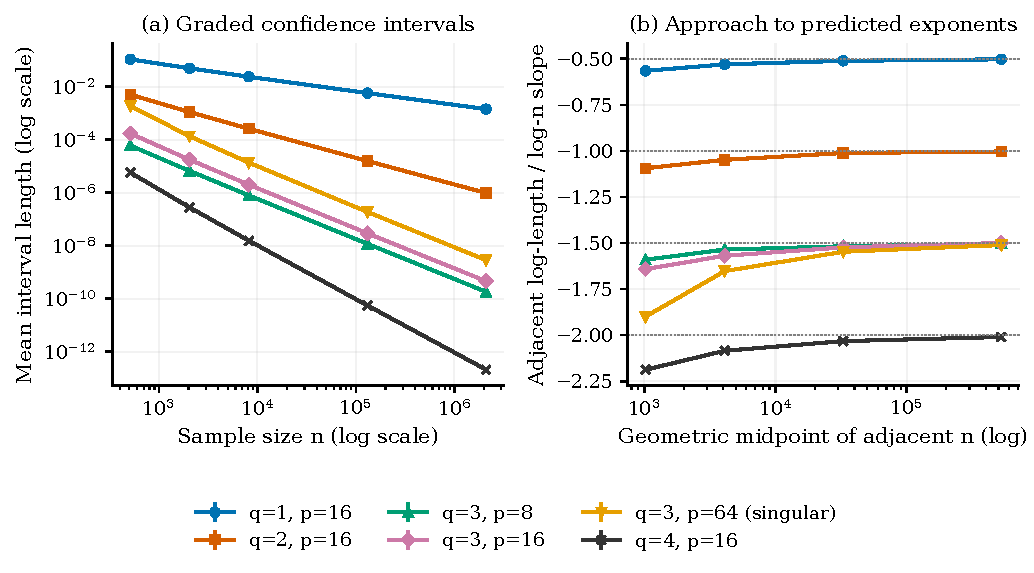
\includegraphics[width=\textwidth]{rates.pdf}
\caption{The graded interval exhibits contact orders one through four, with visible finite-dimension effects before the limiting regime. Each point uses 2,000 Gaussian datasets, $B_0=3E_{00\cdots0}$ and $A=E_{11\cdots1}$; mean-length bars are $\pm1.96$ Monte Carlo standard errors, often smaller than markers. The final two sample sizes are the disclosed addendum, and dotted slope guides mark $-q/2$.}\label{fig:rates}
\end{figure}

All graded intervals in the exactly specified contact experiments cover their targets. This demonstrates substantial conservatism. For example, at $n=2048$ in the four-way three-block setting, the mean graded length is $1.746\times10^{-5}$, compared with $1.741\times10^{-2}$ for the ambient scalar interval and $1.704\times10^{-8}$ for boundary-degree Wald. The last interval has empirical coverage 0.947 at the exact point but is not honest over its neighborhood. These numbers demonstrate a rate gain over ambient inference, not sharp constants or dominance over other valid minimum-distance constructions. In the $q=1$ slack setting, the graded ball is wider than the efficient scalar baseline.

\subsection{Rank activation and two prespecified functionals}
Use the path $B_{n,c}$ from Proposition~\ref{prop:wald}, with $c\in\{0,1,2,4,8\}$, $\lambda=3$ and $\sigma=0.2$. Its second central unfolding singular value is
\[
 \tau_2=\lambda|u_n|(1+u_n^2)
\]
for the values used here. It is zero at the boundary and is the smaller nonzero central singular value for $c>0$. The fixed loadings are
\[
 A_{\rm tan}=\frac{E_{0000}+0.35E_{0110}}{\sqrt{1+0.35^2}},
 \qquad A_{\rm normal}=E_{1111}.
\]
The first is substantially tangent aligned; the second is cubic normal at $c=0$ and nearly normal along the local path. Known-rank Wald uses an original-mode rank-one HOSVD when $c=0$ and the three-block HOSVD when $c>0$. Selected-rank Wald uses the former unless the second central singular value of OLS exceeds $\kappa\sigma\sqrt{2/n}$, with prespecified $\kappa=1,2,3$. These are diagnostic rank selectors, not asserted consistent selectors in a local-signal regime.

At $n=2048,c=2$, normal-loading coverage is 1.000 for graded inversion, 0.849 for known-rank Wald, 0.5525 for selected-rank Wald with $\kappa=2$, and 0.475 for boundary-degree Wald. The last value has Monte Carlo standard error about 0.0112. At $c=0$, its coverage is 0.9535. At $c=8$, it is 0.488, consistent with the approximately 0.4865 iterated limit in Proposition~\ref{prop:wald}. Thus knowledge of the actual rank does not remove functional degeneracy, and exact-boundary calibration does not provide uniform inference. For the tangent loading at $c=2$, corresponding known-rank and selected-$\kappa=2$ coverages are 0.9475 and 0.9255, showing a smaller but visible selection effect.

\subsection{Approximate structure and sensitivity}
For the four-way cubic loading, let $s_n=\tn^3/\lambda^2$. The allowance grid is
\[
 \eta\in\{0,s_n,100s_n,10000s_n,\tn^2/\lambda,\tn\}.
\] We evaluate both $B_0$ and the admissible departure $B_0+\eta A$, comparing exact-model and tube-aware graded intervals. At $n=2048$, $s_n=9.591\times10^{-9}$. A departure $\eta=\tn^2/\lambda=6.510\times10^{-6}$ reduces exact-model graded coverage to 0.847; tube-aware coverage is 1.000. At $\eta=10000s_n$, the exact-model interval has zero empirical coverage, while the tube-aware interval again covers in all replications and increases its mean length to $2.092\times10^{-4}$.

The honest interval's large finite-sample constants delay the visible transition relative to the asymptotic threshold $s_n$. It still covers all tested departures at $100s_n$ even though its exact-model guarantee does not apply there. This is consistent with a rate theorem whose constants are not sharp. Figure~\ref{fig:tube} shows both the cost of a known allowance at the exact point and the coverage consequence of ignoring a departure.

\begin{figure}[t]
\centering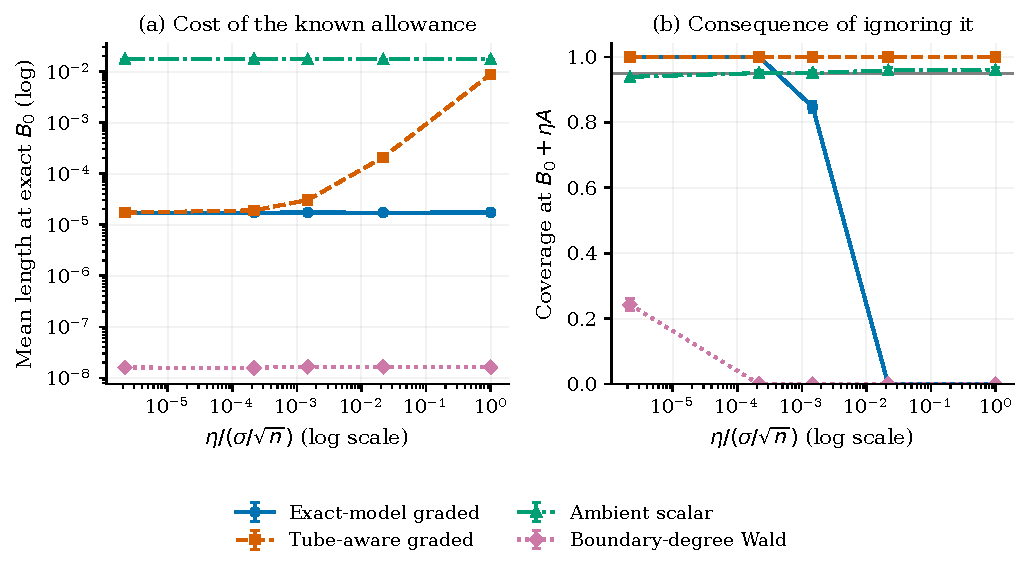
\includegraphics[width=\textwidth]{tube.pdf}
\caption{A known structural allowance increases honest length and protects against departures that invalidate exact-model inference. Four binary modes have caps $(1,2,1)$, $n=2048$, $\lambda=3$, $\sigma=0.2$, and $A=E_{1111}$. The left panel evaluates length at $B_0$ and the right coverage at $B_0+\eta A$, each with 2,000 replications; length bars are $\pm1.96$ Monte Carlo standard errors and coverage bars are Wilson 95\% Monte Carlo intervals.}\label{fig:tube}
\end{figure}

\subsection{Unknown noise, dense signals, and assumption diagnostics}
The study also varies $\lambda\in\{0.5,1,3\}$, rotates the signal and loading densely within modes, uses Gaussian design covariance $\Sigma_{ij}=0.5^{|i-j|}$, and evaluates the residual-$F$ procedure. The latter retains exact conditional coverage under Gaussian homoskedastic errors; a correlated full-rank design does not invalidate that statement. Dense rotations illustrate that coefficient sparsity is not needed.

Separate stress cases use standardized $t_5$ errors, heteroskedastic Gaussian errors, AR(1) errors with correlation 0.6, and Gaussian scale mixtures with 1\% or 5\% outlier probability and outlier standard deviation $5\sigma$. These cases are outside the exact noise theorem. For instance, at 5\% contamination the ambient interval using the uncontaminated $\sigma$ covers only 0.8045, while its residual-$t$ version covers 0.947 in this experiment. Conservative graded coverage at the tested boundary does not establish robustness to any of these departures. All diagnostic results, rather than only favorable settings, are included in the companion tables.

\subsection{Audit addendum: loading transitions and the energy certificate}
After proving the loading-uniform result and energy refinement, we specified a new paired study at $n=512,8192,131072$. Each sample size uses a separate cohort of 2,000 Gaussian datasets at $B_0=3E_{0000}$ with caps $(1,2,1)$ and $\sigma=0.2$. On each dataset we evaluate seven loadings $A_\epsilon$ from Section~\ref{sec:extensions}, setting $\epsilon=\kappa\tn^2/\lambda^2$ for $\kappa\in\{0,0.1,1,10,100,1000,10000\}$. We compare original and improved certificates with known and unknown noise, and the ambient scalar baseline. These are 6,000 additional datasets and 210,000 interval records; loading and method comparisons within a cohort are paired.

The improved length never exceeds the original in any replicate, as Lemma~\ref{lem:energy} predicts. At $n=8192$, $\kappa=0$, the mean lengths are $1.9715\times10^{-6}$ and $4.6578\times10^{-7}$ respectively. Their ratio is $0.23626$ with paired Monte Carlo standard error $0.00041$. Both intervals cover in all 2,000 repetitions, with Wilson interval $[0.9981,1]$. The improved mean length remains about 389 times $\mathcal R_A(\tn)$, so the reduction does not establish sharp confidence constants. At $\kappa=10000$, the ratio increases to $0.99261$ (Monte Carlo standard error $0.00003$), consistent with the tangent term dominating the certificate. Figure~\ref{fig:audit_transition} examines both the multiscale normalization and paired comparison.

\begin{figure}[t]
\centering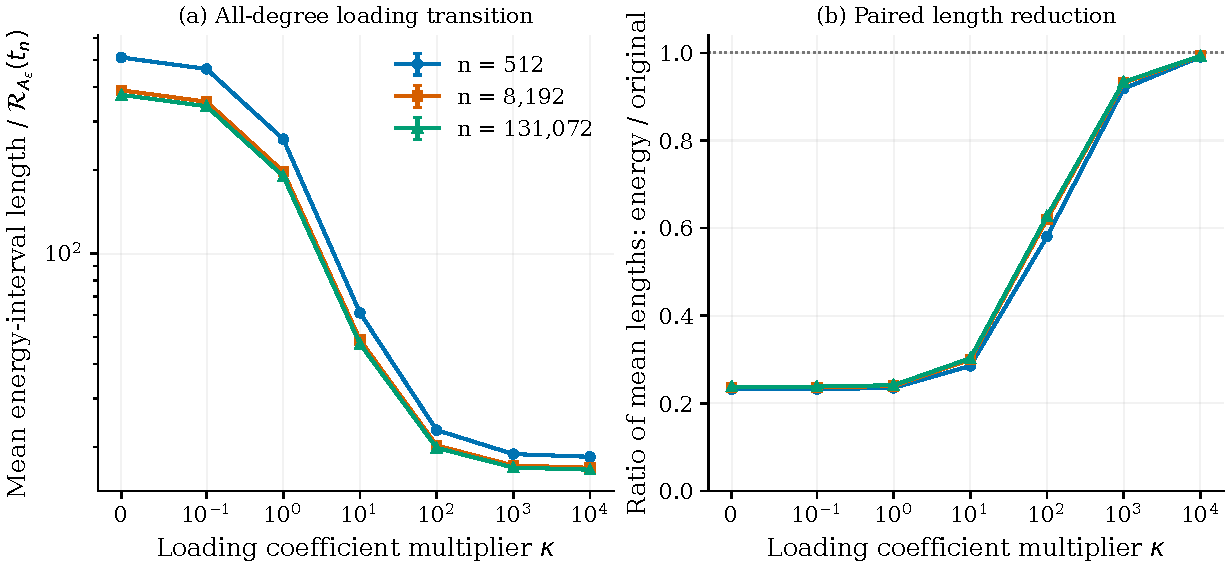
\includegraphics[width=\textwidth]{audit_transition.pdf}
\caption{The energy certificate reduces length while the multiscale normalization tracks loading transitions. The coefficient is $\epsilon=\kappa\tn^2/\lambda^2$ in the prespecified loading $A_\epsilon$. Each sample-size cohort contains 2,000 datasets reused across loadings and methods. Bars are pointwise $\pm1.96$ Monte Carlo standard errors; ratios use paired influence-variable errors. The horizontal line in the right panel is equal mean length. The left panel is normalized by a rate scale, not an exact optimal confidence constant.}\label{fig:audit_transition}
\end{figure}

\subsection{Audit addendum: independent finite-variance noise}
A final study, specified after the proof of Theorem~\ref{thm:robust}, uses independent Gaussian designs, $B_0=3E_{0000}$, $A=E_{1111}$, and a known variance bound $\bar\sigma^2=0.2^2$. The errors are either Gaussian or standardized Student $t_{2.5}$; the latter have finite variance but no finite third or fourth moment. Each noise/sample-size cohort contains 1,000 datasets at $n=512,2048,8192$, and the same observations are used for the $q=3$ and $q=4$ cap profiles. Thus there are 6,000 additional datasets and 12,000 intervals.

Every median-localized interval covers in these runs; the Wilson interval for 1,000 successes is $[0.9962,1]$. Under $t_{2.5}$ noise the fitted mean-length slopes are $-1.598$ and $-2.133$ for $q=3,4$, with Monte Carlo standard errors $0.0010$ and $0.0015$. These slopes remain steeper than $-1.5$ and $-2$ over this finite grid and are not presented as precise asymptotic confirmation. Figure~\ref{fig:robust_audit} displays the finite-sample behavior. The deliberately large variance-bound radius explains the conservatism; the result establishes a proved order under weaker noise assumptions, not a practically efficient robust interval.

\begin{figure}[t]
\centering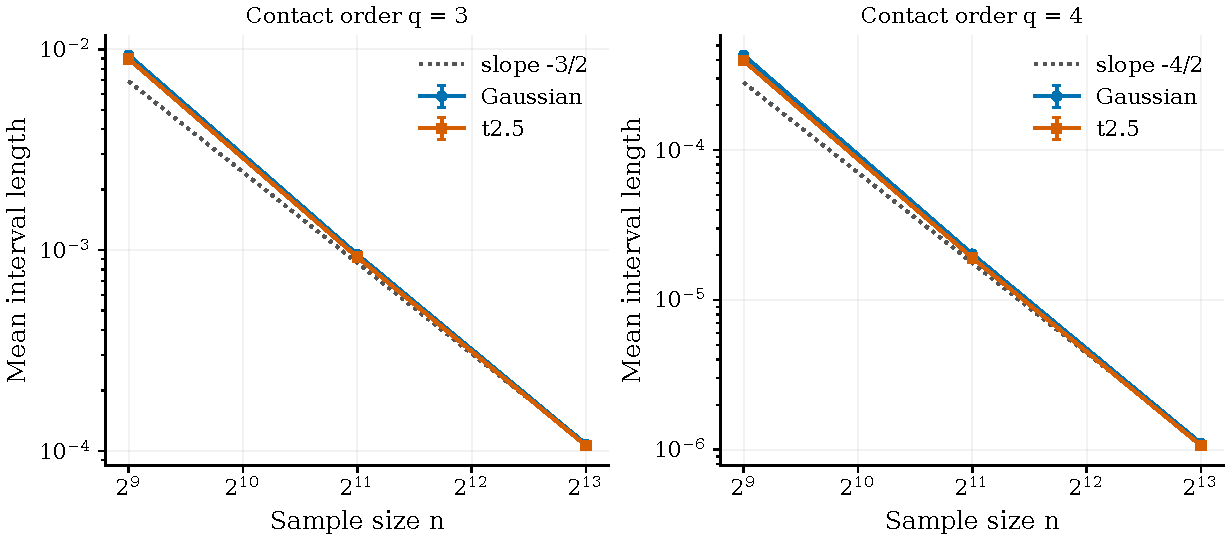
\includegraphics[width=\textwidth]{robust_audit.pdf}
\caption{Median-localized intervals shrink at higher orders under Gaussian and finite-variance heavy-tailed errors. Each point is a mean over 1,000 datasets with $\pm1.96$ Monte Carlo standard-error bars. The $t_{2.5}$ errors have variance $0.2^2$ but lack third and fourth moments. Dotted lines show the predicted limiting slopes, while the observed finite-grid slopes remain steeper. The two cap profiles share observations within each noise/sample-size cohort.}\label{fig:robust_audit}
\end{figure}

\section{Discussion and limitations}
The main conclusion is a loading-uniform local modulus and honest-length formula at original-mode rank-one points in capped TT classes. It retains all orthogonal degrees and therefore describes transitions that an integer contact order alone cannot represent. Cap-one cuts determine the exponent, while internal constraints can leave a singular feasible set without changing that exponent. If every cut permits an additional rank, all nonzero linear functionals return to first order. These statements describe the geometry of the declared class, not a universal benefit of tensor parameterization or rank selection.

The approximation result is consequential for interpretation. A confidence interval with an $n^{-3/2}$ pointwise length relies on a structural allowance of the same order if that gain is to persist uniformly. An ambient coefficient departure of order between $n^{-3/2}$ and $n^{-1/2}$ can be statistically undetectable and still dominate the target uncertainty. The theorem therefore argues for explicit sensitivity analysis whenever rank restrictions are approximate. It does not provide a way to infer the required small allowance from the same sample without additional assumptions.

The limitations are substantial. The pointwise length theorem fixes ambient dimension and uses an original-mode rank-one evaluation point; its constants are uniform over the unit signal directions and deterministic loadings. The OLS ball can incur large dimension constants. Although the energy refinement substantially shortens intervals at a tested cubic point, the experiments still show that it is far from a sharp constant procedure. No matching dimension-dependent minimax length, efficient confidence constant, or general classification at non-rank-one TT points has been established. Coverage for data-selected contrasts follows from the common ball, but the expected-length formula for arbitrary dependent loadings and coverage conditional on selection remain separate questions. The local norm-hardness result does not establish hardness of optimal inference.

\paragraph{Status of possible extensions.}
\textsc{Partial}: growing-dimensional inference has a valid ambient localization construction and fixed-geometry lower bounds, but their dimension factors do not match. \textsc{Conjectured}: a general classification at non-rank-one points with several weak bonds may require higher-order feasible arcs beyond the present elementary paths; no universal rate is asserted. \textsc{Partial}: the spectral-norm reduction identifies a difficult constant but leaves computationally optimal intervals unresolved. \textsc{Proved}: design distributions satisfying explicit Gram conditions and a known conditional second-moment noise bound are treated in Section~\ref{sec:extensions}, with a slower upper bound in the latter case. \textsc{Proved}: Theorem~\ref{thm:robust} retains the full rate for independent observation pairs under a known conditional variance bound. Arbitrary dependence and an unknown unrestricted variance bound do not inherit this result; Counterexample C12 gives a nonshrinking-length obstruction for the latter. Only the statements labeled Partial or Conjectured remain research questions; the proved extensions have explicit assumptions and complete derivations.

\subsection{Relevance to modern AI and why no LLM benchmark is claimed}
A tensor regression head on frozen features offers a direct statistical setting for coefficient functionals. In a locally linear adapter model, a fixed evaluation contrast has the form $\ip{A}{B}$, with $A$ determined by held-out or externally fixed Jacobian features. Existing TT adapters make such restrictions plausible modeling choices, but a trained LLM does not automatically satisfy isotropic design, Gaussian residuals, fixed dimensions, or a known approximation allowance. A fully observed checkpoint is also a deterministic approximation object, not the sampling experiment in \eqref{eq:model}.

Accordingly, this draft contains no real-data or trained-LLM result. The companion application protocol specifies a frozen-feature regression study with a separately fixed functional, sample splitting for any learned loading, residual checks, and an explicit sensitivity grid. A convincing application would need to justify the population target and structural approximation bound, rather than add an LLM benchmark to support a general mathematical claim. The present theory applies independently of any AI interpretation.

\paragraph{Research assessment.}
The completed fixed-dimensional results support a focused theoretical manuscript for further expert evaluation. The central novelty candidate is the cap-profile modulus, now uniform over loading degrees, and its inferential interpretation. Generic higher-order asymptotics and confidence-region inversion remain established tools. A broader theory of local moduli at singular structured parameters, or dimension-dependent optimality with a useful procedure, would be needed to make a strong case for the Annals of Statistics. The current draft should not be treated as submission ready solely because its proofs and experiments are complete.

\paragraph{Reproducibility and proof status.}
The accompanying project includes the full literature matrix, theorem ledger, assumption audit, canonical proof source, fixed-seed simulation code, replicate outputs, vector figures, and a workbook containing the plotted summaries and source metadata. Results marked \pr\ have complete derivations and internal mathematical checks. This label does not certify priority or replace independent mathematical review. The empirical addenda, later supporting local-Wald derivation, and adversarial proof audit are disclosed in the project records. The audit found no false baseline numbered result under its actual assumptions and records proved improvements separately from open extensions.

\clearpage
\bibliography{references}
\clearpage
\appendix
\section{Complete derivations}\label{app:proofs}
Throughout, finite-dimensional norms are Euclidean or Frobenius. Every constant is allowed to depend on the fixed geometry specified in the theorem. The label \pr\ records a complete internal derivation, not independent peer review, a computer-verified proof, or a priority certificate.

\subsection{Product structure at cap-one cuts}
\begin{lemma}\label{lem:blocks}
Every nonzero tensor obeying the cap-one prefix constraints is a product across the induced consecutive blocks. Conversely, if a product of block tensors has within-block TT ranks at most the corresponding internal caps, it belongs to the full capped TT class whenever its norm is at most $M$.
\end{lemma}
\begin{proof}
\emph{Roadmap:} peel successive rank-one unfoldings and check internal ranks. At the first cap-one cut, a nonzero rank-one unfolding factors as a vector for the first block times a vector for the remaining modes. A later prefix unfolding is, up to row ordering, the Kronecker product of the first vector and the corresponding prefix unfolding of the remaining tensor. Multiplication by a nonzero vector preserves rank. The next cap-one constraint therefore factors the remaining tensor again. Induction proves the first assertion. The same rank-preservation calculation shows that an internal unfolding of a block product has the rank of that block's internal unfolding; a block boundary has rank one. This proves the converse. Zero belongs to both classes separately.
\end{proof}

\subsection{Proof of Theorem~\ref{thm:contact}}
\paragraph{Roadmap.} Bound each orthogonal degree separately. For the reverse bound, signed feasible paths isolate any chosen coefficient by a finite Walsh average; this prevents cancellation by smaller degrees. Finally optimize the leading elementary coefficient by an energy inequality.

For a feasible nonzero $B=s\bigotimes_jw_j$ with unit block factors and $\norm{B-B_0}\le t$, projection off $w_j$ gives
\[
 \lambda\sqrt{1-(v_j^\top w_j)^2}\le t,\qquad
 \norm{B_S}\le(\lambda+t)(t/\lambda)^{|S|}.
\]
For degrees zero and one, contractivity of orthogonal projection bounds their pairing with $A$ by $(a_0+a_1)t$. For $\ell\ge2$, the $\binom J\ell$ masks are orthogonal, giving
\[
 |\ip{\Pi_\ell A}{B-B_0}|
 \le a_\ell\binom J\ell^{1/2}(\lambda+t)(t/\lambda)^\ell.
\]
Sum and use $t\le\lambda/2$ to prove the uniform upper bound. Zero is outside this local ball.

For the lower bound extend each original-mode $u_k$ to an orthonormal basis. At degree $\ell\ge1$ the induced elementary products form an orthonormal basis of size
\[
 N_\ell=\sum_{|S|=\ell}\prod_{j\in S}(D_j-1).
\]
If $a_\ell>0$, then $N_\ell>0$ and some mask $S$, $|S|=\ell$, and elementary $w_j\perp v_j$ have coefficient $|c_S|\ge a_\ell/\sqrt{N_\ell}$. For each sign vector $\epsilon\in\{-1,1\}^S$, use the path
\[
 B_\epsilon(s)=\lambda\bigotimes_{j\in S}(v_j+\epsilon_jsw_j)
                         \bigotimes_{j\notin S}v_j,
 \qquad s^2=(1+t^2/\lambda^2)^{1/\ell}-1.
\]
Each internal unfolding has rank at most two, each boundary cut has rank one, and Lemma~\ref{lem:blocks} proves feasibility. Moreover,
\[
 \norm{B_\epsilon(s)-B_0}^2=\lambda^2\{(1+s^2)^\ell-1\}=t^2,
 \qquad \norm{B_\epsilon(s)}=\sqrt{\lambda^2+t^2}<M.
\]
Expand the finite product and average with the top sign character:
\[
 2^{-\ell}\sum_\epsilon\left(\prod_{j\in S}\epsilon_j\right)
       \ip{A}{B_\epsilon(s)-B_0}=\lambda c_Ss^\ell.
\]
Indeed each monomial for a proper subset of $S$ has at least one sign appearing to the first power, whose average is zero. Thus at least one feasible sign choice has absolute target change at least $\lambda|c_S|s^\ell$. The mean value theorem, with $t/\lambda\le1/2$, gives
\[
 s^2\ge\frac{4}{5\ell}(t/\lambda)^2.
\]
Therefore $\omega_{A,0}(t)\ge c_{\ell,D}a_\ell t^\ell/\lambda^{\ell-1}$. If $a_0>0$, the feasible radial path gives $\omega_{A,0}(t)\ge a_0t$. Zero-dimensional degrees simply contribute zero. The maximum of these $J+1$ nonnegative bounds is at least their sum divided by $J+1$. This proves the uniform lower bound with constants independent of the loading and signal directions.

For fixed $A$, the first nonzero degree now implies \eqref{eq:modulus}; higher terms are bounded by its order when $t\le\lambda$. For $t\ge\lambda$, Cauchy--Schwarz gives $\omega_{A,0}(t)\le\norm{A}t\le\norm{A}t^q/\lambda^{q-1}$, proving the global bound. For the pure elementary loading the preceding unsigned path has target $\lambda s^q$, so its scaled limit is $q^{-q/2}$.

For the exact elementary coefficient, use a local product chart for any feasible $B$ within $t<\lambda$:
\[
 B=c\bigotimes_{j=1}^J(v_j+z_j),\quad z_j\perp v_j,
 \quad c=\ip{B}{\bigotimes_jv_j}\ge\lambda-t>0.
\]
Nonzero projections onto every $v_j$ follow from the same positive $c$. Orthogonal expansion gives
\[
 t^2\ge(c-\lambda)^2+c^2\left\{\prod_j(1+\norm{z_j}^2)-1\right\}
 \ge c^2\sum_j\norm{z_j}^2.
\]
For the elementary loading active on $S$, its target is $c\prod_{j\in S}\ip{w_j}{z_j}$. Cauchy--Schwarz and the arithmetic--geometric mean inequality give
\[
 |\ip{A}{B}|\le c\prod_{j\in S}\norm{z_j}
 \le\frac{t^q}{q^{q/2}c^{q-1}}
 \le\frac{t^q}{q^{q/2}(\lambda-t)^{q-1}}.
\]
The unsigned elementary path has the matching leading coefficient. For $q=1$ it also attains the exact Cauchy--Schwarz bound $t$. This proves every claim of the theorem.

\subsection{Proof of Proposition~\ref{prop:slack} and the singular example}
\paragraph{Roadmap.} Add a rank-one direction at a slack point; inspect determinantal minors for the separate singularity example.
Choose a unit elementary original-mode product $H$ with $\ip{A}{H}\ne0$, which exists because elementary products span the ambient space. Rank subadditivity gives
\[
 \rank((B+sH)^{[k]})\le\rank(B^{[k]})+1\le\bar r_k.
\]
For $|s|<M-\norm{B}$ the norm constraint also holds. This gives the lower bound $|\ip{A}{H}|t$; Cauchy--Schwarz gives the upper bound.

In the six-mode example, the middle block has dimensions $2\times2\times2\times2$. The internal edge unfoldings have rank at most two automatically. Its central $4\times4$ unfolding is constrained to rank at most two, a proper determinantal variety. At a rank-one point this variety is singular: the differentials of all its $3\times3$ minors vanish, so its algebraic tangent space is the full 16-dimensional space, whereas the dimension of the rank-at-most-two variety is $2(4+4-2)=12$. Factoring the two external nonzero lines gives a local product chart with this variety; its singularity persists. The elementary path in the preceding proof remains feasible and gives cubic contact. For any one prefix cut with cap one, the corresponding elementary contrast is perpendicular on both matrix sides and the two-factor calculation gives order two. At the other cuts cap two leaves rank-one slack, giving order one. This verifies the stated scope of the matrix comparison.

\subsection{Information bound and tube geometry}
\begin{lemma}[Two-point expected-length bound]\label{lem:twopoint}
If an interval has coverage at least $1-\alpha$ at $B_0$ and $B_1$, then
\[
 \E_{B_0,\sigma}|I|\ge|\ip{A}{B_1-B_0}|
 \left[1-2\alpha-\frac{\sqrt n\norm{B_1-B_0}}{2\sigma}\right]_+.
\]
\end{lemma}
\begin{proof}
\emph{Roadmap:} compute Gaussian relative entropy, convert to total variation, and force simultaneous inclusion of two targets. The design distributions are identical at the two coefficients. Conditional Gaussian relative entropy equals $\norm{X(b_1-b_0)}^2/(2\sigma^2)$; its expectation under isotropic design is $n\norm{b_1-b_0}^2/(2\sigma^2)$. Pinsker's inequality therefore bounds total variation by $\sqrt n\norm{b_1-b_0}/(2\sigma)$. Under $B_0$, the event that the interval contains both target values has probability at least $1-2\alpha-\TV$. On that event its length is at least their separation. Integrating proves the bound. This is the usual two-point modulus argument, not a new information inequality.
\end{proof}

For a unit loading, compactness of $\Th_0$ and Cauchy--Schwarz give the tube sandwich, for small $t$ with $\lambda+t<M$:
\begin{equation}\label{eq:tubesandwich}
 \max\{\omega_{A,0}(t),\eta\wedge t\}
 \le\omega_{A,\eta}(t)
 \le\min\{t,\eta+\omega_{A,0}(t+\eta)\}.
\end{equation}
Indeed $\Th_0\subseteq\Th_\eta$ and $B_0+(\eta\wedge t)A$ supplies the two lower bounds. For any feasible $B$, choose a nearest $B^\dagger\in\Th_0$. Then $\norm{B-B^\dagger}\le\eta$ and $\norm{B^\dagger-B_0}\le t+\eta$, proving the upper bound. For a nonunit loading the corresponding factors are $\norm{A}$, which are absorbed in constants. If $\eta\le t$, Theorem~\ref{thm:contact} and $(t+\eta)^q\le2^qt^q$ give an upper bound of order $\eta+t^q/\lambda^{q-1}$. If $\eta>t$, use the upper bound $t$. The lower bounds combine via $\max(x,y)\ge(x+y)/2$.

Take $h=1-2\alpha>0$ and $t=h\tn$ in Lemma~\ref{lem:twopoint}. Its bracket is at least $h/2$. A supremizing local alternative, or a sequence approaching the supremum, gives the lower bound in Theorem~\ref{thm:length}, using \eqref{eq:tubesandwich}. The signal condition ensures these alternatives stay within the norm cap. For unknown $\sigma$, restricting the honest procedure to alternatives with this same $\sigma$ proves exactly the same lower bound. At a slack point Proposition~\ref{prop:slack} and the same lemma give a root-$n$ lower bound, matched by ambient inference.

For Corollary~\ref{cor:pretest}, the explicit alternative is within $\eta_n$ of $B_0$ and its norm is below $M$ eventually. The entropy calculation yields $\KL=\eta_n^2/(2\tn^2)\to0$, while its target separation is $\eta_n$. Apply the two-point bound. The argument applies to any measurable interval, including those obtained after an arbitrary rank pretest.

\subsection{Localization and moment control}
\begin{lemma}[Gaussian OLS localization]\label{lem:OLS}
Both radii in Section~\ref{sec:method} give conditional coverage at least $1-\alpha$ when $X$ has full column rank. Under isotropic Gaussian design, for fixed $p,J,\alpha$ and $n\ge p+m$, $m=\max(J,2)$, for every integer $1\le k\le\max(J,2)$,
\[
 \E\norm{z-b}^k+\E e^k\le C_k(\sigma/\sqrt n)^k.
\]
\end{lemma}
\begin{proof}
\emph{Roadmap:} use orthogonal Gaussian projections for coverage, then explicit inverse-chi-square moments for expectations. Conditional on $X$, $S^{1/2}(z-b)/\sigma$ is standard normal, and hence $\norm{z-b}^2\le\sigma^2\chi_p^2/\lambda_{\min}(S)$ under a coupling. The squared residual norm divided by $\sigma^2$ is independent $\chi^2_{n-p}$ by orthogonal Gaussian projections. The normalized squared Mahalanobis error divided by $p\widehat\sigma^2$ is therefore $F_{p,n-p}$. These facts prove both coverage statements.

Here are details ensuring the expectation bound does not discard a localization failure event. Write $S=X^\top X\sim W_p(n,I)$. The reciprocal of $(S^{-1})_{jj}$ is the squared norm of column $j$ after projecting off the other $p-1$ columns. Conditioning on those columns shows it has law $\chi^2_{\nu}$, $\nu=n-p+1$. For $a>0$ with $\nu>2a$,
\[
 \E(\chi_\nu^2)^{-a}=2^{-a}\frac{\Gamma(\nu/2-a)}{\Gamma(\nu/2)}.
\]
For fixed $a=k/2$, integer $1\le k\le m$, and integer $\nu\ge m+1$, this is at most $C_a\nu^{-a}$: the gamma-ratio asymptotic proves boundedness after multiplication by $\nu^a$ at infinity, and continuity bounds it on the remaining finite set of integer degrees of freedom. In particular $\nu>k$, so the gamma argument is positive. This use of the gamma ratio involves fixed moment order only. Since $\lambda_{\min}(S)^{-1}\le\operatorname{tr}(S^{-1})$, for $a\ge1$ the inequality $(\sum_jx_j)^a\le p^{a-1}\sum_jx_j^a$ gives
\[
 \E\lambda_{\min}(S)^{-a}\le C_{a,p}n^{-a}.
\]
For $0<a<1$, Jensen's inequality and $\E\operatorname{tr}(S^{-1})=p/(n-p-1)$ give the same conclusion. Conditional Gaussian moments now bound $\E\norm{z-b}^k$ by $C_{k,p}\sigma^k\E\lambda_{\min}(S)^{-k/2}$.

The residual scale has $k$th moment bounded by $C_k\sigma^k$, uniformly in $n-p\ge1$, and is independent of $S$ since its conditional distribution does not depend on $X$. The fixed upper quantiles $F_{p,n-p;1-\alpha}$ are bounded over integers $n-p$ bounded away from zero: their distributions converge to $\chi_p^2/p$, and the finite initial set has finite quantiles. Thus the known- and unknown-noise radii have the asserted moment bounds. Here $\nu=n-p+1\ge m+1>k$, and $n/(n-p-1)\le(p+m)/(m-1)$; these facts justify the uniform constants used above. The original condition $n\ge2p+2J+8$ is unnecessary. The revised condition is sufficient, not necessary for the interval itself.
\end{proof}

\begin{lemma}[HOSVD pilot and changing block projectors]\label{lem:pilot}
Let $\widehat B$ be the rank-one HOSVD approximation to $Z$. For every block-product $B_0$,
\[
 \norm{Z-\widehat B}\le\sqrt J\norm{Z-B_0},\qquad
 h:=\norm{\widehat B-B_0}\le(1+\sqrt J)\norm{Z-B_0}.
\]
If $h<\lambda/2$ and $A$ has no true block components of degree below $q\ge1$, then
\begin{equation}\label{eq:mixing}
 \norm{\widehat\Pi_\ell A}\le C_J\norm{A}
 (h/\lambda)^{(q-\ell)_+},\qquad 0\le\ell\le J.
\end{equation}
For $q=1$ with a radial loading component, only the trivial bounds needed below are asserted.
\end{lemma}
\begin{proof}
\emph{Roadmap:} telescope commuting projections, then count cross-line factors in each pair of masks. Let $\widehat P_j$ be the leading left-singular-vector projection in mode $j$. It minimizes the mode-$j$ rank-one projection residual, which is at most $\norm{Z-B_0}$ because the true block line is an admissible competitor. The commuting orthogonal projections have the telescoping expansion
\[
 Z-\prod_j\widehat P_j Z
 =\sum_j\left(\prod_{i<j}\widehat P_i\right)(I-\widehat P_j)Z.
\]
Terms are orthogonal: for terms $j<k$, the first lies in the complement of the $j$th line and the second lies in that line. Summing squared norms proves the first bound; the triangle inequality proves the second.

Projection of $B_0-\widehat B$ off the pilot line in block $j$ gives $\lambda\sin\theta_j\le h$. The two cross-line operators satisfy $\norm{\widehat P_jQ_j}_{\rm op}=\norm{(I-\widehat P_j)P_j}_{\rm op}=\sin\theta_j$. If a true mask $S$ has size at least $q$ and a pilot mask $T$ has size $\ell<q$, then $|S\setminus T|\ge q-\ell$. The tensor product of mask operators therefore has operator norm at most $(h/\lambda)^{q-\ell}$; all other factors have norm at most one. Sum over the at most $2^{2J}$ pairs of masks and use $\sum_S\norm{A_S}\le2^{J/2}\norm{A}$. For $\ell\ge q$, use the contractivity of an orthogonal projection. These steps establish \eqref{eq:mixing} with a finite $J$-dependent constant.
\end{proof}

\subsection{Proof of Theorem~\ref{thm:procedure}}
\paragraph{Roadmap.} Prove coverage on one simultaneous ball event. Bound length on a localized pilot event and control its complement by moments, without replacing probability bounds by expectation claims.
On the OLS ball event, take a closest $B^\dagger\in\Th_0$ to the true $B\in\Th_\eta$. Compactness ensures existence, and
\[
 \norm{B^\dagger-\widehat B}\le\eta+\norm{B-z}+\norm{z-\widehat b}\le\rho.
\]
By Lemma~\ref{lem:blocks}, $B^\dagger$ is in the block-product envelope. If $\rho<\widehat s/2$, write it in the pilot chart as $c\bigotimes_j(\widehat v_j+z_j)$, where $z_j\perp\widehat v_j$ and $c\ge\widehat s-\rho>0$. Its orthogonal expansion implies $c^2\sum_j\norm{z_j}^2\le\rho^2$. Lemma~\ref{lem:energy} bounds the combined degree-$\ell$ norm by $\kappa_{J,\ell}\rho^\ell/(\widehat s-\rho)^{\ell-1}$. Replacing $\kappa_{J,\ell}$ by the larger $\binom J\ell^{1/2}$ also proves the original certificate used in the primary simulations. The degree-zero and degree-one part of $B^\dagger-\widehat B$ has norm at most $\rho$. Pairing with the corresponding loading projections proves the second expression in \eqref{eq:graded}; Cauchy--Schwarz proves the first. The fallback is valid for the same reason. The difference between the true and projected targets is at most $\eta\norm{A}$. Thus $I_s$ contains the true target on the ball event. So does $I_a$. Their intersection is nonempty and contains it on that event. This proves conditional coverage, without any independence between pilot and ball. The ball event is independent of the choice of loading, and the argument on it holds for every $A$. Substitution of any measurable data-selected $\widehat A$ therefore proves the simultaneous-coverage assertion for the random target. Conditioning further on its selected value is not justified by this argument.

It remains to prove expected length, not merely length on a favorable event. At $B_0$, put $r=\norm{z-b_0}$ and $T=r+e$. Lemma~\ref{lem:pilot} gives
\[
 h\le(1+\sqrt J)r,\quad \norm{z-\widehat b}\le\sqrt J r,
 \quad\rho\le(1+\sqrt J)(T+\eta).
\]
First let $\eta\le\tn$. Choose a fixed small $c_J>0$ so that on $G=\{T+\eta\le c_J\lambda\}$, $h\le\lambda/8$, $\rho\le\lambda/8$, and $\widehat s-\rho\ge3\lambda/4$. When $q\ge2$, \eqref{eq:mixing} bounds the first part of \eqref{eq:graded} by
\[
 C\norm{A}(h/\lambda)^{q-1}\rho
 \le C\norm{A}(T+\eta)^q/\lambda^{q-1}.
\]
For $2\le\ell<q$, the same inequality bounds its $\ell$th summand by
\[
 C\norm{A}(h/\lambda)^{q-\ell}\rho^\ell/\lambda^{\ell-1}
 \le C\norm{A}(T+\eta)^q/\lambda^{q-1}.
\]
For $\ell\ge q$, use $\rho/\lambda\le1$ to reach the same bound. For $q=1$ use $H\le\norm{A}\rho$ directly, including a nonzero radial component. Thus on $G$, $H\le C\norm{A}(T+\eta)^q/\lambda^{q-1}$.

On $G^c$ the definition always gives $H\le\norm{A}\rho\le C\norm{A}(T+\eta)$. Moreover
\[
 (T+\eta)\one_{G^c}\le
 \frac{(T+\eta)^q}{(c_J\lambda)^{q-1}},
\]
also for $q=1$. Lemma~\ref{lem:OLS}, $\eta\le\tn$, and $(x+y)^q\le2^{q-1}(x^q+y^q)$ now yield
\[
 \E|I|\le2\eta\norm{A}+2\E H
 \le C\{\eta+\tn^q/\lambda^{q-1}\}.
\]
If $\eta>\tn$, intersection with $I_a$ gives $|I|\le2e\norm{A}$ (the empty case has zero length), so its expectation is at most $C\tn$. This establishes the fixed-degree assertion for every $\eta$. For the loading-uniform assertion use Theorem~\ref{thm:transfer} with $r_n=\tn$ and $m=\max(J,2)$; its proof below decomposes all true loading degrees and controls the bad event degree by degree. Lemma~\ref{lem:OLS} verifies every required moment. To finish the uniform lower bound in Theorem~\ref{thm:length}, apply the tube sandwich with its explicit $\norm{A}$ factors and the uniform part of Theorem~\ref{thm:contact}. For $h=1-2\alpha$, each term of $\mathcal R_A(h\tn)$ is at least $h^J$ times its term at $\tn$, and $\min(\eta,h\tn)\ge h\min(\eta,\tn)$. The two-point bracket is at least $h/2$. The maximum of the structural and tube lower bounds is at least half their sum. All constants are independent of $A$ and the unit factors.

\subsection{Proof of Proposition~\ref{prop:hardness}}
\paragraph{Roadmap.} Bound the cubic form by its injective norm and realize a maximizing product direction.
In the local chart $B=c(e_0+x)\otimes(e_0+y)\otimes(e_0+z)$, each vector is perpendicular to $e_0$. The target equals $c\ip{T}{x\otimes y\otimes z}$. The energy bound gives $c^2(\norm{x}^2+\norm{y}^2+\norm{z}^2)\le t^2$. Hence
\[
 |\ip{A}{B}|\le c\norm{T}_{\rm inj}\norm{x}\norm{y}\norm{z}
 \le\frac{\norm{T}_{\rm inj}t^3}{3\sqrt3(\lambda-t)^2}.
\]
Compactness of the unit spheres gives maximizing directions for $\norm{T}_{\rm inj}$. The product path with those directions and $s^2=(1+t^2/\lambda^2)^{1/3}-1$ is feasible in the three-block product class and attains the matching limit. Setting $\lambda=1$ identifies the squared spectral norm with 27 times the squared modulus coefficient. Thus an oracle evaluating this coefficient exactly also evaluates a known NP-hard tensor quantity as dimensions vary. The reduction adds no claim about approximation factors beyond those established for that source problem.

\subsection{Proof of Proposition~\ref{prop:wald}}
\paragraph{Roadmap.} Derive the OLS Gaussian limit, solve the HOSVD eigenvector equation to first order, and apply the monomial distribution only at the exact boundary.
Under the triangular sequence $B_{n,c}$, the OLS error distribution is independent of the coefficient. The law of large numbers gives $S/n\to I$ in probability, and conditional normality implies
\[
 (z-b_{n,c})/\tn\xrightarrow{d}G,\qquad G\sim N_p(0,I).
\]
This implication can be verified directly from conditional characteristic functions:
\[
 \E[\exp\{-h^\top(nS^{-1})h/2\}]\to\exp(-\norm{h}^2/2),
\]
by bounded convergence in probability. Expand $B_{n,c}=B_0+c\tn\sum_{j=1}^3 E_j+O(\tn^2/\lambda)$, where $E_j$ changes the designated coordinate in exactly block $j$. These three elementary tensors are orthonormal.

For completeness, the required HOSVD first-order expansion follows from its eigenvector equation. In any block unfolding, $Z=\lambda e_0w_0^\top+\tn D_n$, with $D_n=O_P(1)$, so
\[
 ZZ^\top=\lambda^2e_0e_0^\top+
 \lambda\tn(e_0g_n^\top+g_ne_0^\top)+O_P(\tn^2),\quad g_n=D_nw_0.
\]
Weyl's bound, obtained here from the Rayleigh variational formula, places the largest eigenvalue at $\lambda^2+O_P(\tn)$ and all other eigenvalues at $O_P(\tn)$. Choose the leading unit eigenvector with positive first coordinate, and write it $a_ne_0+h_n$, $h_n\perp e_0$. Projecting its eigenvector equation orthogonally to $e_0$ first gives $h_n=O_P(\tn/\lambda)$, then substitution gives
\[
 h_n=(\tn/\lambda)(I-e_0e_0^\top)g_n+O_P(\tn^2/\lambda^2),
 \qquad a_n=1+O_P(\tn^2/\lambda^2).
\]
Indeed the projected linear operator on $h_n$ has inverse norm $O_P(\lambda^{-2})$, and the cross block is $\lambda\tn(I-e_0e_0^\top)g_n+O_P(\tn^2)$, which justifies both substitutions. The HOSVD scalar coefficient equals $\lambda+O_P(\tn)$. The designated perpendicular coordinate in block $j$ therefore equals $(\tn/\lambda)(c+Z_{n,j})+o_P(\tn/\lambda)$, where jointly $Z_{n,j}\to Z_j$ and their independence follows from the orthonormal $E_j$ coordinates of $G$.

Contracting the pure-normal loading with the fitted product yields the asserted product limit. For its tangent projection, the leading terms are the three mutually orthogonal $E_j$ directions, with coefficients
\[
 (\tn/\lambda)^2\prod_{k\ne j}(c+Z_{n,k})+o_P(\tn^2/\lambda^2).
\]
The radial term is of order $(\tn/\lambda)^3$; perturbing the remaining unit directions changes the leading terms only by a smaller order. Since $nS^{-1}\to I$, the standard-error limit follows.

The limiting denominator is positive almost surely. The equality boundary of the coverage event has probability zero: after squaring, it is the zero set of a nonzero polynomial in a Gaussian vector. To see the latter fact without a regularity assumption, induct on dimension, condition on all but one coordinate, and use that a nonzero univariate polynomial has finitely many roots; the exceptional coefficient-zero sets are treated by the induction hypothesis. Thus convergence in distribution gives convergence of coverage probabilities. At $c=0$ apply the cited monomial law. Finally, as $c\to\infty$,
\[
 \frac{\prod_j(c+Z_j)-c^3}
 {\{\sum_j\prod_{k\ne j}(c+Z_k)^2\}^{1/2}}
 =\frac{Z_1+Z_2+Z_3}{\sqrt3}+o_P(1).
\]
This follows by dividing numerator and denominator by $c^2$ and expanding the finite products. The displayed iterated limits now follow from the standard normal distribution. No uniform-in-$c$ approximation or arbitrary growing-$c_n$ limit is asserted.

\section{Strengthened certificates and localization transfer}\label{app:strengthening}
\begin{lemma}[Energy bound for every block degree]\label{lem:energy}
Let $B^\dagger$ be a block product within Frobenius distance $\rho<\widehat s$ of $\widehat B=\widehat s\bigotimes_j\widehat v_j$, where $\widehat s>0$ and the factors are unit vectors. For $2\le\ell\le J$,
\[
 \norm{\widehat\Pi_\ell B^\dagger}
 \le\binom J\ell^{1/2}J^{-\ell/2}
                \frac{\rho^\ell}{(\widehat s-\rho)^{\ell-1}}.
\]
Consequently the improved interval has length no greater than the original interval on every dataset, with the same fallback and empty-intersection conventions.
\end{lemma}
\begin{proof}
\emph{Roadmap:} keep the sum of squared block perturbations, bound the elementary symmetric polynomial by averaging coordinates, and compare the two nested structured intervals.
Use the chart $B^\dagger=c\bigotimes_j(\widehat v_j+z_j)$, with $c\ge\widehat s-\rho>0$ and $z_j\perp\widehat v_j$. Set $x_j=\norm{z_j}^2$. Orthogonal expansion gives $c^2\sum_jx_j\le\rho^2$ and
\[
 \norm{\widehat\Pi_\ell B^\dagger}^2=c^2 e_\ell(x),
 \qquad e_\ell(x)=\sum_{|S|=\ell}\prod_{j\in S}x_j.
\]
For nonnegative $x$ of sum $u$, compactness gives a maximum of $e_\ell$. If $u=0$, the assertion is immediate. If $u>0$, the maximum is positive for $\ell\le J$, and any maximizer has at least $\ell$ positive coordinates. Replacing an unequal pair $x_i,x_j$ by their average preserves their sum and increases their product strictly. In the identity
\[
 e_\ell(x)=e_\ell(x_{-i,-j})+(x_i+x_j)e_{\ell-1}(x_{-i,-j})
                         +x_ix_je_{\ell-2}(x_{-i,-j}),
\]
we use $e_0=1$ and $e_k=0$ above the number of coordinates. The last coefficient is positive at a positive maximizer: after removing any unequal pair there remain at least $\ell-2$ positive coordinates. Thus an unequal pair contradicts maximality. All coordinates are equal, proving
$e_\ell(x)\le\binom J\ell(u/J)^\ell$.
Substitute $u\le\rho^2/c^2$ and take square roots to obtain the bound.

The improved coefficients are no larger than the original ones, so their structured intervals are nested and have identical centers. Intersecting each with the same ambient interval preserves containment when both intersections are nonempty. If the improved intersection is empty its reported length is zero. If the original intersection is empty then the improved one is also empty. In every case the improved length is no greater. The fallback coefficients are identical. This is a deterministic length comparison, not equality of coverage probabilities or optimality of the resulting constants.
\end{proof}

\subsection{Proof of Theorem~\ref{thm:transfer}}
\paragraph{Roadmap.} Coverage is deterministic on the confidence-ball event. For expected length decompose the loading into its true degrees, use cross-projector mixing on a localized event, and truncate each degree at the available moment order on its complement.
The coverage proof of Theorem~\ref{thm:procedure} only uses the ball event and product geometry, so it applies verbatim, with no distributional step left to check. A nearest point exists because $\Th_0$ is compact.

Write $T=\norm{z-b_0}+e$, $U=T+\eta$, and $G=\{U\le c_J\lambda\}$ for the same sufficiently small $c_J$ as in that proof. Decompose $A=\sum_{\ell=0}^J A^{(\ell)}$, $A^{(\ell)}=\Pi_\ell A$, $\norm{A^{(\ell)}}=a_\ell$, and put $k_\ell=\max(1,\ell)$. On $G$ the graded expression before its minimum is subadditive in $A$, by the triangle inequality for each projected norm. For a single pure degree, Lemma~\ref{lem:pilot} and the term-by-term calculation in the procedure proof give
\[
 H(A)\one_G\le C\sum_{\ell=0}^J a_\ell
           \frac{U^{k_\ell}}{\lambda^{k_\ell-1}}\one_G
 \le C\sum_{\ell=0}^J a_\ell
           \frac{U^{d_\ell}}{\lambda^{d_\ell-1}}\one_G.
\]
The first inequality uses the graded expression as an upper bound for $H$; it does not assume that a minimum of norms is subadditive. The second uses $U/\lambda\le c_J\le1$ and $d_\ell\le k_\ell$. For degree zero and degree one, every projected loading norm is at most $a_\ell$. Their graded expressions are consequently at most
\[
 a_\ell\rho\left\{1+\sum_{r=2}^J\kappa_{J,r}
       \left(\frac{\rho}{\widehat s-\rho}\right)^{r-1}\right\}
 \le C_Ja_\ell\rho,
\]
since $\rho/(\widehat s-\rho)\le1/6$ on $G$. The same bound holds for the original larger coefficients. This bounds each graded expression itself, without substituting a bound for its minimum. On $G^c$,
\[
 H(A)\le\norm{A}\rho\le C\sum_\ell a_\ell U,
 \qquad U\one_{G^c}\le
        U^{d_\ell}/(c_J\lambda)^{d_\ell-1}
\]
for each $\ell$, including $d_\ell=1$. Hence the same sum of moment powers bounds $H$ on the whole sample space. If $\eta\le r_n$, the assumed moments and $(x+y)^k\le2^{k-1}(x^k+y^k)$ give $\E U^k\le C'_k r_n^k$ for all $k\le m$. Since $|I|\le2H+2\eta\norm{A}$, this proves the desired bound in this case. If $\eta>r_n$, ambient intersection gives $|I|\le2e\norm{A}$, including the zero-length empty case; the first moment bound finishes the proof. No stochastic-order statement is used as a substitute for integrability.

\subsection{Proof of Corollary~\ref{cor:design}}
\paragraph{Roadmap.} Retain the exact conditional Gaussian pivot, check localization moments using the assumed inverse Gram moments, and replace the isotropic relative-entropy identity by an upper bound.
Conditional on $X$, let $G\sim N_p(0,I_p)$ represent $S^{1/2}(z-b)/\sigma$. Its conditional law is constant, so $G$ is independent of $X$ in this representation. Then
\[
 \E\norm{z-b}^k\le\sigma^k\E\norm{G}^k\,
                            \E\lambda_{\min}(S)^{-k/2}
 \le C'_k\tn^k.
\]
The known radius has the same moment bound. Orthogonal Gaussian projections show that $\widehat\sigma/\sigma$ has law $\sqrt{\chi^2_{n-p}/(n-p)}$, independent of $X$ and of the standardized OLS error. Its positive moments are bounded uniformly in the positive integer $n-p$. For fixed $p,\alpha$, the $F$ upper quantiles are bounded over those integers, by convergence to $\chi_p^2/p$ and the finite initial set. Thus the unknown radius has the same bounds. Theorem~\ref{thm:transfer} proves the upper result.

For any coefficient difference $\delta$, the common design law and conditional normality give
\[
 \operatorname{KL}(P_{b_0},P_{b_0+\delta})
 =\frac{\delta^\top(\E S)\delta}{2\sigma^2}
 \le\frac{Ln\norm{\delta}^2}{2\sigma^2}.
\]
Choose local radius $(1-2\alpha)\tn/\max(1,\sqrt L)$ in the two-point lemma and use the uniform modulus and tube lower bounds. The changed constants depend on $L$ only in addition to the earlier constants.
For deterministic bounded Gram matrices the assumptions follow by direct eigenvalue bounds. For Gaussian rows with covariance $\Sigma$, write $S=\Sigma^{1/2}W\Sigma^{1/2}$, where $W\sim W_p(n,I)$. Then $\lambda_{\min}(S)\ge\lambda_{\min}(\Sigma)\lambda_{\min}(W)$ and $\E S=n\Sigma$. Lemma~\ref{lem:OLS} supplies the moment conditions when $n\ge p+\max(J,2)$ and $\Sigma$ has the stated eigenvalue bounds. This verifies the examples without asserting that an arbitrary full-rank design has good moments.

\subsection{Proof of Proposition~\ref{prop:variance}}
\paragraph{Roadmap.} Compute a conditional second moment, use Markov's inequality on its square, and transfer the first two localization moments.
OLS has error $S^{-1}X^\top\varepsilon$, conditional mean zero, and covariance at most $\bar\sigma^2S^{-1}$. Therefore
\[
 \E(\norm{z-b}^2\mid X)\le\bar\sigma^2\operatorname{tr}(S^{-1}),
 \qquad
 \PP(\norm{z-b}>e_{\rm v}\mid X)\le\alpha.
\]
The interval coverage follows from Theorem~\ref{thm:transfer}. If the trace moment condition holds, then
\[
 \E(\norm{z-b_0}+e_{\rm v})^2
 \le2\bar\sigma^2(1+\alpha^{-1})\E\operatorname{tr}(S^{-1})
 \le C'\bar\sigma^2/n.
\]
Cauchy--Schwarz supplies the first moment. Apply that theorem with $m=2$. No third or higher error moment, Gaussian projection independence, or residual variance consistency has been assumed.

\subsection{Proof of Corollary~\ref{cor:unbounded}}
\paragraph{Roadmap.} Replace global compactness by bounded minimizing sequences for distance, then inspect every use of the norm cap.
The TT class is closed because each unfolding rank constraint is the simultaneous zero set of its minors. It contains zero. For any finite $B$, a minimizing sequence $C_k$ for distance to this class has $\norm{B-C_k}\le\norm B+1$ eventually, hence $\norm{C_k}\le2\norm B+1$. A subsequence converges in finite dimension, its limit remains in the closed class, and continuity attains the distance. The tube is closed since distance to a nonempty set is a 1-Lipschitz function.
The modulus upper bounds use product structure only; all signed and radial witness paths remain feasible without the norm restriction. The two-point alternatives remain admissible. The coverage proof requires an attained nearest point, now supplied above. HOSVD localization, projector mixing, and all moment calculations make no use of $M$. These observations verify each proof under the enlarged parameter spaces, with identical constants. At $B_0=0$ the local-signal assumption fails and the contact classification is not extended.

\subsection{Proof of Theorem~\ref{thm:robust}}
\paragraph{Roadmap.} Bound one coordinate of each group OLS estimate by a second-moment calculation, amplify its tail through independent groups, integrate the amplified tail through order $J$, and invoke the localization transfer theorem. The Gaussian submodel supplies the matching lower bound.
Let $z^{(s)}$ be OLS in group $s$, with Gram matrix $S_s$. Given all designs in that group, conditional means of the errors are zero and conditional cross covariances vanish, because the observation pairs are independent. The diagonal conditional variances are at most $\bar\sigma^2$. Thus
\[
 \E\{(z_j^{(s)}-b_j)^2\mid X_s\}
 \le\bar\sigma^2(S_s^{-1})_{jj},\qquad
 \E(z_j^{(s)}-b_j)^2
 \le\frac{\bar\sigma^2}{k-p-1}\le\frac{2\bar\sigma^2}{k}.
\]
The middle identity for the inverse Gram expectation follows from the same residualized-column chi-square integral as Lemma~\ref{lem:OLS}; $k\ge2p+2$ verifies both its finiteness and the last inequality. For every $v>0$, Markov's inequality gives
$\PP(|z_j^{(s)}-b_j|>v)\le2\bar\sigma^2/(kv^2)$, uniformly over the noise law and $b$.

If the median of $g=2h-1$ numbers differs from $b_j$ by more than $v$, at least $h$ of those numbers differ in absolute value by more than $v$. The group estimates are independent, although their coordinates within a group need not be. A union over the $\binom gh$ subsets of size $h$, followed by a union over $p$ coordinates with $v=u/\sqrt p$, gives
\[
 \PP(\norm{z_{\rm med}-b}>u)
 \le\min\left\{1,\ p\binom gh
       \left(\frac{2p\bar\sigma^2}{ku^2}\right)^h\right\}
 =\min\{1,(D/u)^{2h}\}.
\]
This verifies the unconditional confidence ball at $u=e_{\rm med}$. No simultaneous-coordinate independence or Gaussian error tail is used. For every real $0<r<2h$, tail integration gives
\[
 \E\norm{z_{\rm med}-b}^r
 =\int_0^\infty r u^{r-1}\PP(\norm{z_{\rm med}-b}>u)\,du
 \le D^r+\frac{rD^r}{2h-r}
 =\frac{2h}{2h-r}D^r.
\]
Here $2h>J$, so the integer moments through $J$ are finite. Also $n/g\ge2$ and $k=\lfloor n/g\rfloor\ge n/(2g)$, hence $D\le C_{p,J}\bar\sigma/\sqrt n$. Since $e_{\rm med}$ is deterministic, the sum $\norm{z_{\rm med}-b}+e_{\rm med}$ has all required moments through $J$ with uniform constants. Apply Theorem~\ref{thm:transfer} with $m=J$, $r_n=\bar t_n$, and the median ball to obtain coverage and the length upper bound.

For the lower bound take the admissible conditional noise law $Q_G=N(0,\bar\sigma^2)$ independent of the design. Every procedure honest for all $Q$ is honest on this Gaussian submodel. The two-point calculation at noise scale $\bar\sigma$, the uniform loading modulus, and the tube alternative give the lower scale in the display. The supremum over $Q$ in expected length is at least its value at $Q_G$. Taking the infimum over honest procedures preserves the bound. This proof uses the direct lower-bound argument, so it does not require importing the Gaussian procedure's separate sufficient sample-size threshold. The median upper bound is uniform over $Q$, completing the comparison.

\section{Counterexamples and boundaries of the conclusions}\label{app:counterexamples}
These examples test proposed relaxations. They do not contradict the stated theorems.

\paragraph{C1: zero signal changes the order.}
At $B_0=0$ any elementary rank-one $H$ gives a feasible path $sH$ under every positive cap profile. For nonzero $A$, choose $H$ with $\ip A H\ne0$. Then $\omega_{A,0}(t;0)\asymp t$, including classes with several cap-one cuts. Thus the order $t^q/\lambda^{q-1}$ cannot be continued through $\lambda=0$. More generally $\omega\le\norm A t$, so a higher-order formula cannot hold without a local restriction on $t/\lambda$.

\paragraph{C2: uncertain validity of cap-one restrictions.}
In four binary modes, $B_0=\lambda E_{0000}$ and $A=E_{1111}$ have cubic contact under caps $(1,2,1)$. If the honesty class instead permits caps $(2,2,2)$, the path $B_0+sE_{1111}$ is feasible and changes the target by $s$. The root-$n$ two-point lower bound then applies. Choosing the smaller caps from the same data does not remove the larger-class alternatives.

\paragraph{C3: an unobserved structured direction.}
For a two-mode coefficient with cap one, consider $B_\theta=\theta E_{11}$ and a design satisfying $X_{i,11}=0$ almost surely. Distinct $\theta$ produce exactly the same data distribution, although all coefficients in this submodel have rank at most one. The coordinate functional is not identifiable. Thus full ambient identifiability can be weakened to injectivity on structured differences, but no such injectivity assumption can simply be omitted. This example does not assert impossibility for every structured model with $p\ge n$.

\paragraph{C4: independent-error scaling cannot cover arbitrary dependence.}
Take scalar regression with $X_i=1$ and errors $\varepsilon_i=Z$ for all $i$, where $Z\sim N(0,\sigma^2)$. Then $z-b=Z$ does not shrink, whereas residual variance is zero. The residual-$F$ interval is the singleton $\{z\}$ and has zero coverage for $b$. This example embeds in $K\ge2$ by taking all mode dimensions one. Its error covariance has largest eigenvalue $n\sigma^2$, violating the bounded conditional covariance assumption in Proposition~\ref{prop:variance}.

\paragraph{C5: finite variance does not give the Gaussian pivot.}
For $p=1$, $n=2$ and fixed $X=(1,0)^\top$, let the first error be zero with probability $0.9$ and equal to $\pm\sqrt{10}\sigma$ with probability $0.05$ each; take the second error independently with the same distribution. These errors have mean zero and variance $\sigma^2$. The known-Gaussian 95\% radius is $1.96\sigma$ and its coverage is $0.9$. The variance-bound radius in Proposition~\ref{prop:variance} avoids this failure. This is a finite-sample pivot counterexample, not a claim that asymptotic Gaussian approximation is impossible under finite variance.

\paragraph{C6: pointwise order does not imply a loading-uniform rate.}
Let $A_\epsilon=(E_{1111}+\epsilon E_{1000})/\sqrt{1+\epsilon^2}$ at the four-way cubic point. For every $\epsilon>0$, its contact order is one. If $\epsilon=t^2/\lambda^2$, however, Theorem~\ref{thm:contact} gives $\omega_{A_\epsilon,0}(t)\asymp t^3/\lambda^2$. There cannot be a positive loading-uniform lower constant multiplying $t$ based solely on the label $q=1$. The multiscale statement repairs this limitation rather than assigning a discontinuous statistical rate to an arbitrarily small coefficient.

\paragraph{C7: pointwise coverage alone has no positive length bound.}
The deterministic interval $\{\psi_A(B_0)\}$ covers at $B_0$ with probability one and has zero length. It generally fails elsewhere. Every information lower bound in this paper therefore uses honesty at alternatives as well as at $B_0$.

\paragraph{C8: full rank does not control inverse design moments.}
Take $p=1$, $X_1=\sqrt n V$, $X_i=0$ for $i>1$, and $V$ uniform on $(0,1)$. The design has full column rank almost surely and $\E S=n/3$, but $\E S^{-1/2}=\infty$. The known Gaussian confidence-ball radius has infinite expectation. Finite-sample conditional coverage still holds. This distinguishes invertibility from the sufficient moment condition in Corollary~\ref{cor:design}; it does not prove those particular moments necessary for every possible procedure. For a separate information counterexample, take deterministic $X_i=1/n$, so $S=1/n$ despite full rank. Two fixed scalar coefficients separated by $\delta$ have Gaussian total variation at most $|\delta|/(2\sigma\sqrt n)$. Honesty at both therefore forces expected length at least $|\delta|(1-2\alpha-o(1))$. Full rank alone cannot guarantee a shrinking $n^{-1/2}$ length.

\paragraph{C9: favorable probability events do not imply fast expected length.}
For any $q>1$, a nonnegative variable equal to $n^{-q/2}$ with probability $1-n^{-1/2}$ and to one otherwise is $O_P(n^{-q/2})$, but its expectation is of order $n^{-1/2}$. The bad-event moment calculation in Theorem~\ref{thm:transfer} is therefore essential. No uniform-integrability step is left implicit.

\paragraph{C10: a higher-order ordinary bootstrap can fail.}
In the scalar Gaussian mean experiment at $\theta=0$, $\sqrt n\bar Y=Z_n\sim N(0,1)$. For the squared-mean target and a parametric bootstrap $\bar Y^*=\bar Y+Z^*/\sqrt n$, the true statistic is $n\bar Y^2=Z_n^2$, but conditionally
\[
 n\{(\bar Y^*)^2-\bar Y^2\}=2Z_nZ^*+(Z^*)^2.
\]
At any fixed $z\ne0$, this bootstrap expression is negative with probability $\Phi(2|z|)-1/2>0$, whereas the target chi-square law is nonnegative. Since $Z_n$ does not converge to zero in probability, the conditional discrepancy persists with positive probability. No bootstrap validity is claimed for the tensor interval; this example illustrates why a generic bootstrap substitution would require a separate proof.

\paragraph{C11: scalar validity does not imply post-selection validity.}
In an orthogonal Gaussian mean experiment with $Z_1,\ldots,Z_p$ independent standard normal at the zero coefficient, choose the coordinate with largest $|Z_j|$. The usual coordinatewise 95\% interval covers the selected zero target only when $\max_j|Z_j|\le z_{.975}$, which has probability $0.95^p$. The common-ball intervals avoid this problem because their coverage argument holds simultaneously for all loadings. They still do not assert coverage conditional on an arbitrary selection event.

\paragraph{C12: no uniform shrinking interval over all unknown variance bounds.}
The known upper bound in Theorem~\ref{thm:robust} cannot simply be replaced by an unspecified finite bound while retaining distribution-free honesty. Here is an explicit regression version of the classical nonparametric impossibility mechanism associated with \citet{bahadur1956}; no external theorem is needed for the argument.
Fix a baseline $Y\mid x\sim N(x^\top b_0,\sigma_0^2)$ and any alternative coefficient $b_1=b_0+\delta$ in the declared class. For $0<\epsilon<1$, let
\[
 w_\epsilon(x)=\min\{1,\epsilon[1+(x^\top\delta)^2]\}.
\]
At the alternative, take the conditional response law
\[
 (1-w_\epsilon)N(x^\top b_0,\sigma_0^2)
 +w_\epsilon N(x^\top b_0+x^\top\delta/w_\epsilon,\sigma_0^2).
\]
Its conditional mean is $x^\top b_1$. Its conditional error variance is
\[
 \sigma_0^2+\frac{1-w_\epsilon}{w_\epsilon}(x^\top\delta)^2
 \le\sigma_0^2+\epsilon^{-1},
\]
a finite uniform bound for each $\epsilon$, although these bounds grow as $\epsilon\downarrow0$. With iid Gaussian designs the one-observation total variation from the baseline is at most $\E w_\epsilon\le\epsilon(1+\norm\delta^2)$; coupling independent observations bounds the $n$-observation distance by $n$ times this quantity. Therefore, for fixed $n$, honesty over every finite variance bound implies
\[
 \PP_{B_0,\sigma_0}\{\psi_A(B_1)\in I\}\ge1-\alpha
\]
by sending $\epsilon\downarrow0$ in the coverage inequality at $B_1$.
Let $\mathcal T=\{\psi_A(B):B\in\Th_0\}$. The bounded TT class is symmetric and closed under scaling toward zero, so $\mathcal T$ is an interval; it has positive length for nonzero $A$, since an elementary product has a nonzero coefficient. Tonelli's theorem applied to interval membership gives
\[
 \E_{B_0,\sigma_0}|I|\ge\int_{\mathcal T}
       \PP_{B_0,\sigma_0}\{t\in I\}\,dt
 \ge(1-\alpha)\operatorname{length}(\mathcal T).
\]
This nonshrinking bound holds for every $n$. For the unbounded rank class, $\mathcal T=\R$ and the expected length is infinite. The conclusion concerns honesty uniformly over all finite conditional variance bounds, not pointwise asymptotic inference for a fixed noise law or the Gaussian unknown-variance model.

\end{document}
